\documentclass[12pt, a4paper]{article}

% ------------------------------ font
\usepackage{times} %pdflatex
% \usepackage{luatexja}
% \usepackage{luatexja-fontspec}

% \setmainfont{Times New Roman}
% \setmainjfont[BoldFont=IPAexGothic]{IPAexMincho}
\usepackage{color}
\newcommand{\revise}[1]{{\color{red}{#1}}}

% ------------------------------ math
\usepackage{amsmath,amssymb}
\usepackage{siunitx}

% ------------------------------ author & natbib
\usepackage{authblk}
\usepackage[semicolon]{natbib}
\bibliographystyle{agsm}

% ------------------------------ appendix
\usepackage[title]{appendix}

% ------------------------------ tables
\usepackage{here}
\usepackage{longtable, booktabs, array}
\usepackage{threeparttable, threeparttablex, multirow}
% \newcolumntype{d}{S[input-symbols = ()]}
\usepackage{lscape}

% ------------------------------- figures
\usepackage[labelfont=bf, labelsep=period, justification=justified]{caption}
\usepackage{graphics, graphicx}
\makeatletter
\def\maxwidth{\ifdim\Gin@nat@width>\linewidth\linewidth\else\Gin@nat@width\fi}
\def\maxheight{\ifdim\Gin@nat@height>\textheight\textheight\else\Gin@nat@height\fi}
\makeatother
% Scale images if necessary, so that they will not overflow the page
% margins by default, and it is still possible to overwrite the defaults
% using explicit options in \includegraphics[width, height, ...]{}
\setkeys{Gin}{width=\maxwidth,height=\maxheight,keepaspectratio}

% ------------------------------ page settings
\usepackage[left=3cm,right=3cm,top=3cm,bottom=3cm]{geometry}
\usepackage{setspace}
\renewcommand{\baselinestretch}{1.5}
\providecommand{\tightlist}{%
  \setlength{\itemsep}{0pt}\setlength{\parskip}{0pt}}

% ------------------------------ hyperlink
\usepackage[hidelinks]{hyperref}

% ------------------------------ other packages
\usepackage{booktabs}
\usepackage{siunitx}

  \newcolumntype{d}{S[
    input-open-uncertainty=,
    input-close-uncertainty=,
    parse-numbers = false,
    table-align-text-pre=false,
    table-align-text-post=false
  ]}
  

% ------------------------------ paper information
\title{Online Supplementary Material
``Field experiment Using Text Messages to Promote Stem Cell Donation in Japan Marrow Donor Program''}
\author{}
\date{}

\makeatletter
\renewcommand*{\@fnsymbol}[1]{\ifcase#1\or*\else\@arabic{\numexpr#1-1\relax}\fi}
\makeatother

\begin{document}
\begin{spacing}{1}
  \maketitle
  \end{spacing}



\setcounter{footnote}{0}
\listoftables
\clearpage

\appendix

\setcounter{figure}{0}
\setcounter{table}{0}
\renewcommand\thefigure{\thesection\arabic{figure}}
\renewcommand{\thetable}{\thesection\arabic{table}}
\renewcommand{\theHfigure}{\thesection\arabic{figure}}
\renewcommand{\theHtable}{\thesection\arabic{table}}

\hypertarget{figtab}{%
\section{Additional Figures and Tables}\label{figtab}}

\begin{table}[H]

\caption{\label{tab:assignment}Assignment Schedule}
\centering
\fontsize{8}{10}\selectfont
\begin{threeparttable}
\begin{tabular}[t]{lcccccc}
\toprule
week & September, 2021 & October, 2021 & November, 2021 & December, 2021 & January, 2022 & February, 2022\\
\midrule
1 & B & C & C & D & B & A\\
 & (09/06 to 09/12) & (10/04 to 10/10) & (11/01 to 11/07) & (11/29 to 12/05) & (01/03 to 01/09) & (01/31 to 02/06)\\
2 & D & B & A & A & C & B\\
 & (09/13 to 09/19) & (10/11 to 10/17) & (11/08 to 11/14) & (12/06 to 12/12) & (01/10 to 01/16) & (02/07 to 02/13)\\
3 & A & D & B & C & D & C\\
 & (09/20 to 09/26) & (10/18 to 10/24) & (11/15 to 11/21) & (12/13 to 12/19) & (01/17 to 01/23) & (02/14 to 02/20)\\
4 & C & A & D & B & A & D\\
 & (09/27 to 10/03) & (10/25 to 10/31) & (11/22 to 11/28) & (12/20 to 12/26) & (01/24 to 01/30) & (02/21 to 02/27)\\
\bottomrule
\end{tabular}
\begin{tablenotes}
\item \emph{Note}: See Table 1 in the main manuscrpit for a detailed description of the intervention of each experimental arm. The control arm is experimental arm A. The experiment was not conducted during the week beginning December 27, 2021, and ending January 3, 2022, because JMDP was closed for the New Year's holiday.
\end{tablenotes}
\end{threeparttable}
\end{table}

\hypertarget{balance-test}{%
\subsection{Balance Test}\label{balance-test}}

\begin{table}[H]

\caption{\label{tab:summary}Summary of Field Experiment}
\centering
\fontsize{8}{10}\selectfont
\begin{threeparttable}
\begin{tabular}[t]{lccccc}
\toprule
\multicolumn{1}{c}{ } & \multicolumn{4}{c}{Experimental Arms} & \multicolumn{1}{c}{ } \\
\cmidrule(l{3pt}r{3pt}){2-5}
 & A & B & C & D & F-test, p-value\\
\midrule
\addlinespace[0.3em]
\multicolumn{6}{l}{\textbf{A. Interventions}}\\
\hspace{1em}Standard notification & X & X & X & X & \\
\hspace{1em}Probability message &  & X &  & X & \\
\hspace{1em}Early coordination message &  &  & X & X & \\
\addlinespace[0.3em]
\multicolumn{6}{l}{\textbf{B. Sample Size}}\\
\hspace{1em}N & 2535 & 3053 & 2726 & 2735 & \\
\addlinespace[0.3em]
\multicolumn{6}{l}{\textbf{C. Balance Test}}\\
\hspace{1em}Male (= 1) & 0.624 & 0.633 & 0.631 & 0.609 & 0.231\\
\hspace{1em}Age & 38.376 & 38.121 & 37.448 & 37.978 & 0.004\\
\hspace{1em}Number of past coordination & 1.609 & 1.589 & 1.625 & 1.563 & 0.130\\
\hspace{1em}Number of listed hospitals & 0.476 & 0.490 & 0.487 & 0.485 & 0.835\\
\hspace{1em}Number of hospitals listed with PBSC collection & 0.162 & 0.167 & 0.166 & 0.164 & 0.838\\
\hspace{1em}Number of hospitals listed with BM collection & 0.246 & 0.256 & 0.254 & 0.251 & 0.741\\
\hspace{1em}Number of holidays in the assigned week & 4.544 & 6.329 & 4.466 & 4.770 & 0.000\\
\bottomrule
\end{tabular}
\begin{tablenotes}
\item \emph{Note}: For the balance test, we regressed a covariate on treatment dummies and tested the null hypothesis that all coefficients are zero. We used robust standard errors for statistical inference.
\end{tablenotes}
\end{threeparttable}
\end{table}

\begin{table}[H]

\caption{\label{tab:smd-balance}Assessing Balance by Standaridized Mean Difference}
\centering
\fontsize{8}{10}\selectfont
\begin{threeparttable}
\begin{tabular}[t]{lccc}
\toprule
\multicolumn{1}{c}{ } & \multicolumn{3}{c}{A versus} \\
\cmidrule(l{3pt}r{3pt}){2-4}
\multicolumn{1}{c}{ } & \multicolumn{1}{c}{B} & \multicolumn{1}{c}{C} & \multicolumn{1}{c}{D} \\
\cmidrule(l{3pt}r{3pt}){2-2} \cmidrule(l{3pt}r{3pt}){3-3} \cmidrule(l{3pt}r{3pt}){4-4}
 & (1) & (2) & (3)\\
\midrule
Age & -0.026 & -0.096 & -0.041\\
Male (= 1) & 0.019 & 0.016 & -0.031\\
Number of holidays in the assigned week & 1.073 & -0.129 & 0.317\\
Number of hospitals listed with BM collection & 0.028 & 0.023 & 0.013\\
Number of hospitals listed with PBSC collection & 0.023 & 0.019 & 0.011\\
Number of listed hospitals & 0.024 & 0.019 & 0.015\\
Number of past coordination & -0.019 & 0.015 & -0.045\\
\bottomrule
\end{tabular}
\begin{tablenotes}
\item \emph{Note}: These values represent the standardized mean differences (SMD) with the control arm (experimental arm A). Generally, covariates between two groups are balanced if the SMD is less than $0.1$.
\end{tablenotes}
\end{threeparttable}
\end{table}

\hypertarget{effect-on-the-ct}{%
\subsection{Effect on the CT}\label{effect-on-the-ct}}

\hypertarget{average-treatment-effects}{%
\subsubsection{Average Treatment Effects}\label{average-treatment-effects}}

\begin{table}[H]

\caption{\label{tab:lm-test}Linear Probability Model of the CT}
\centering
\fontsize{8}{10}\selectfont
\begin{threeparttable}
\begin{tabular}[t]{>{\raggedright\arraybackslash}p{20em}cc}
\toprule
\multicolumn{1}{c}{ } & \multicolumn{2}{c}{CT} \\
\cmidrule(l{3pt}r{3pt}){2-3}
  & (1) & (2)\\
\midrule
Treatment B & \num{3.10}*** & \num{3.18}**\\
 & (\num{1.14}) & (\num{1.27})\\
Treatment C & \num{1.19} & \num{0.88}\\
 & (\num{1.16}) & (\num{1.15})\\
Treatment D & \num{2.39}** & \num{2.63}**\\
 & (\num{1.17}) & (\num{1.16})\\
\midrule
Control average & 22.25 & 22.25\\
Covariates &  & X\\
Num.Obs. & \num{11049} & \num{11049}\\
\bottomrule
\end{tabular}
\begin{tablenotes}
\item \emph{Note}: * $p < 0.1$, ** $p < 0.05$, *** $p < 0.01$. The robust standard errors are in parentheses. The unit of treatment effect is a percentage point. Covariates are gender, (demeaned) age, its squared term, the number of past coordinations, the number of public holidays in the assigned week and the following week, the number of hospitals per 10 square kilometers, the number of hospitals with PBSC collection per 10 square kilometers and the number of hospitals with BM collection per 10 square kilometers. All covariates except gender were demeaned.
\end{tablenotes}
\end{threeparttable}
\end{table}

\begin{table}[H]

\caption{\label{tab:logit-test}Logit Model of the CT}
\centering
\fontsize{8}{10}\selectfont
\begin{threeparttable}
\begin{tabular}[t]{>{\raggedright\arraybackslash}p{20em}cc}
\toprule
\multicolumn{1}{c}{ } & \multicolumn{2}{c}{CT} \\
\cmidrule(l{3pt}r{3pt}){2-3}
  & (1) & (2)\\
\midrule
Treatment B & \num{1.19} & \num{1.20}\\
 & {}[\num{1.05}, \num{1.34}] & {}[\num{1.04}, \num{1.38}]\\
Treatment C & \num{1.07} & \num{1.05}\\
 & {}[\num{0.94}, \num{1.22}] & {}[\num{0.93}, \num{1.20}]\\
Treatment D & \num{1.14} & \num{1.16}\\
 & {}[\num{1.01}, \num{1.30}] & {}[\num{1.02}, \num{1.32}]\\
\midrule
Covariates &  & X\\
Num.Obs. & \num{11049} & \num{11049}\\
Log.Lik. & \num{-6083.783} & \num{-5953.670}\\
\bottomrule
\end{tabular}
\begin{tablenotes}
\item \emph{Note}: We show odds ratios and associated 95 percent confidential intervals in square brackets. Covariates are gender, (demeaned) age, its squared term, the number of past coordinations, the number of public holidays in the assigned week and the following week, the number of hospitals per 10 square kilometers, the number of hospitals with PBSC collection per 10 square kilometers and the number of hospitals with BM collection per 10 square kilometers. All covariates except gender were demeaned.
\end{tablenotes}
\end{threeparttable}
\end{table}

\begin{table}[H]

\caption{\label{tab:lm-test-initial}Linear Probability Model of the CT (Only First-time Matched Candidates)}
\centering
\fontsize{8}{10}\selectfont
\begin{threeparttable}
\begin{tabular}[t]{>{\raggedright\arraybackslash}p{20em}cc}
\toprule
\multicolumn{1}{c}{ } & \multicolumn{2}{c}{CT} \\
\cmidrule(l{3pt}r{3pt}){2-3}
  & (1) & (2)\\
\midrule
Treatment B & \num{2.51}* & \num{1.84}\\
 & (\num{1.34}) & (\num{1.51})\\
Treatment C & \num{-0.83} & \num{-0.93}\\
 & (\num{1.35}) & (\num{1.35})\\
Treatment D & \num{1.94} & \num{1.93}\\
 & (\num{1.36}) & (\num{1.37})\\
\midrule
Control average & 18.67 & 18.67\\
Covariates &  & X\\
Num.Obs. & \num{7016} & \num{7016}\\
\bottomrule
\end{tabular}
\begin{tablenotes}
\item \emph{Note}: * $p < 0.1$, ** $p < 0.05$, *** $p < 0.01$. The robust standard errors are in parentheses. The unit of treatment effect is a percentage point. We restricted the analysis sample to those who matched the first time. Covariates are gender, (demeaned) age, its squared term, the number of past coordinations, the number of public holidays in the assigned week and the following week, the number of hospitals per 10 square kilometers, the number of hospitals with PBSC collection per 10 square kilometers and the number of hospitals with BM collection per 10 square kilometers. All covariates except gender were demeaned.
\end{tablenotes}
\end{threeparttable}
\end{table}

\begin{table}[H]

\caption{\label{tab:lm-test-noskip}Linear Probability Model of the CT (Excluding Those Who Skipped the CT)}
\centering
\fontsize{8}{10}\selectfont
\begin{threeparttable}
\begin{tabular}[t]{>{\raggedright\arraybackslash}p{20em}cc}
\toprule
\multicolumn{1}{c}{ } & \multicolumn{2}{c}{CT} \\
\cmidrule(l{3pt}r{3pt}){2-3}
  & (1) & (2)\\
\midrule
Treatment B & \num{2.59}** & \num{2.81}**\\
 & (\num{1.10}) & (\num{1.24})\\
Treatment C & \num{0.61} & \num{0.49}\\
 & (\num{1.12}) & (\num{1.11})\\
Treatment D & \num{1.58} & \num{1.69}\\
 & (\num{1.13}) & (\num{1.13})\\
\midrule
Control average & 19.12 & 19.12\\
Covariates &  & X\\
Num.Obs. & \num{10547} & \num{10547}\\
\bottomrule
\end{tabular}
\begin{tablenotes}
\item \emph{Note}: * $p < 0.1$, ** $p < 0.05$, *** $p < 0.01$. The robust standard errors are in parentheses. The unit of treatment effect is a percentage point. We excluded those who skipped the CT. Covariates are gender, (demeaned) age, its squared term, the number of past coordinations, the number of public holidays in the assigned week and the following week, the number of hospitals per 10 square kilometers, the number of hospitals with PBSC collection per 10 square kilometers and the number of hospitals with BM collection per 10 square kilometers. All covariates except gender were demeaned.
\end{tablenotes}
\end{threeparttable}
\end{table}

\hypertarget{heterogeneous-treatment-effects}{%
\subsubsection{Heterogeneous Treatment Effects}\label{heterogeneous-treatment-effects}}

\begin{table}[H]

\caption{\label{tab:lm-interaction-gender-test}Heterogenous Message Effects on CT by Gender}
\centering
\fontsize{8}{10}\selectfont
\begin{threeparttable}
\begin{tabular}[t]{>{\raggedright\arraybackslash}p{20em}cc}
\toprule
\multicolumn{1}{c}{ } & \multicolumn{2}{c}{CT} \\
\cmidrule(l{3pt}r{3pt}){2-3}
  & (1) & (2)\\
\midrule
Treatment B & \num{2.73} & \num{2.61}\\
 & (\num{1.78}) & (\num{1.95})\\
Treatment C & \num{1.60} & \num{0.95}\\
 & (\num{1.81}) & (\num{1.80})\\
Treatment D & \num{4.91}*** & \num{4.96}***\\
 & (\num{1.83}) & (\num{1.83})\\
Male & \num{4.58}*** & \num{5.63}***\\
 & (\num{1.67}) & (\num{1.94})\\
Treatment B $\times$ Male & \num{0.52} & \num{0.91}\\
 & (\num{2.31}) & (\num{2.56})\\
Treatment C $\times$ Male & \num{-0.71} & \num{-0.10}\\
 & (\num{2.35}) & (\num{2.33})\\
Treatment D $\times$ Male & \num{-4.01}* & \num{-3.87}\\
 & (\num{2.37}) & (\num{2.36})\\
\midrule
Covariates &  & X\\
Num.Obs. & \num{11049} & \num{11049}\\
\bottomrule
\end{tabular}
\begin{tablenotes}
\item \emph{Note}: * $p < 0.1$, ** $p < 0.05$, *** $p < 0.01$. The robust standard errors are in parentheses. This table tests heterogenous message effects by gender. The unit of treatment effect is a percentage point. Covariates are age, the number of past coordinations, the number of public holidays in the assigned week and the following week, the number of hospitals per 10 square kilometers, the number of hospitals with PBSC collection per 10 square kilometers and the number of hospitals with BM collection per 10 square kilometers. All covariates were demeaned. We also controlled cross terms of each covariate and gender.
\end{tablenotes}
\end{threeparttable}
\end{table}

\begin{table}[H]

\caption{\label{tab:lh-interaction-gender-test}Linear Combination Test: Message Effects on the CT for Specific Gender Group}
\centering
\fontsize{8}{10}\selectfont
\begin{threeparttable}
\begin{tabular}[t]{>{\raggedright\arraybackslash}p{8em}>{\raggedright\arraybackslash}p{8em}cc}
\toprule
\multicolumn{2}{c}{ } & \multicolumn{2}{c}{CT} \\
\cmidrule(l{3pt}r{3pt}){3-4}
Group & Treatment & (1) & (2)\\
\midrule
Female & B & 2.73 (1.78) & 2.61 (1.95)\\
 & C & 1.60 (1.81) & 0.95 (1.80)\\
 & D & 4.91 (1.83)*** & 4.96 (1.83)***\\
Male & B & 3.25 (1.48)** & 3.52 (1.65)**\\
 & C & 0.90 (1.50) & 0.85 (1.48)\\
 & D & 0.89 (1.51) & 1.08 (1.49)\\
\midrule
 & Covariates &  & X\\
\bottomrule
\end{tabular}
\begin{tablenotes}
\item \emph{Note}: * $p < 0.1$, ** $p < 0.05$, *** $p < 0.01$. The robust standard errors are in parentheses. We performed a linear combination test on the coefficients of the linear probability model presented in Table \ref{tab:lm-interaction-gender-test}. The null hypothesis for females is that the treatment dummy is zero. The null hypothesis for males is that the sum of the treatment dummy and the cross term of the treatment dummy and the gender dummy is zero.
\end{tablenotes}
\end{threeparttable}
\end{table}

\begin{table}[H]

\caption{\label{tab:mh-adjust-gender-test}Adjustment of p-values for Multiple Testing of Effect on the CT for Specific Gender Group}
\centering
\fontsize{8}{10}\selectfont
\begin{threeparttable}
\begin{tabular}[t]{llccc}
\toprule
\multicolumn{3}{c}{ } & \multicolumn{2}{c}{p-values} \\
\cmidrule(l{3pt}r{3pt}){4-5}
Group & Treatment & Diff-in-mean & Unadjusted & Adjusted\\
\midrule
Female & B & 2.731 & 0.124 & 0.380\\
Female & C & 1.603 & 0.378 & 0.742\\
Female & D & 4.907 & 0.007 & 0.038\\
Male & B & 3.254 & 0.027 & 0.119\\
Male & C & 0.897 & 0.544 & 0.769\\
Male & D & 0.893 & 0.562 & 0.562\\
\bottomrule
\end{tabular}
\begin{tablenotes}
\item \emph{Note}: To adjust p-values for multiple testing, we employed the method proposed by List et al. (2019). For calculation of p-values, we used the bootstrapping with 3,000 boostrap samples.
\end{tablenotes}
\end{threeparttable}
\end{table}

\begin{table}[H]

\caption{\label{tab:lm-interaction-gender-age-test}Heterogenous Message Effects on CT by Gender-Age Group}
\centering
\fontsize{8}{10}\selectfont
\begin{threeparttable}
\begin{tabular}[t]{>{\raggedright\arraybackslash}p{20em}cc}
\toprule
\multicolumn{1}{c}{ } & \multicolumn{2}{c}{CT} \\
\cmidrule(l{3pt}r{3pt}){2-3}
  & (1) & (2)\\
\midrule
Treatment B & \num{2.67} & \num{2.28}\\
 & (\num{2.46}) & (\num{2.68})\\
Treatment C & \num{2.64} & \num{1.57}\\
 & (\num{2.49}) & (\num{2.43})\\
Treatment D & \num{5.72}** & \num{5.63}**\\
 & (\num{2.55}) & (\num{2.53})\\
Older female & \num{-0.67} & \num{-3.19}\\
 & (\num{2.56}) & (\num{2.65})\\
Young male & \num{4.98}** & \num{3.32}\\
 & (\num{2.39}) & (\num{2.46})\\
Older male & \num{3.62} & \num{-0.53}\\
 & (\num{2.31}) & (\num{2.38})\\
Treatment B $\times$ Older female & \num{0.09} & \num{0.55}\\
 & (\num{3.57}) & (\num{3.92})\\
Treatment C $\times$ Older female & \num{-2.59} & \num{-1.74}\\
 & (\num{3.64}) & (\num{3.61})\\
Treatment D $\times$ Older female & \num{-1.80} & \num{-1.52}\\
 & (\num{3.67}) & (\num{3.66})\\
Treatment B $\times$ Young male & \num{1.13} & \num{0.29}\\
 & (\num{3.27}) & (\num{3.56})\\
Treatment C $\times$ Young male & \num{-3.07} & \num{-1.88}\\
 & (\num{3.27}) & (\num{3.22})\\
Treatment D $\times$ Young male & \num{-7.44}** & \num{-6.99}**\\
 & (\num{3.34}) & (\num{3.30})\\
Treatment B $\times$ Older male & \num{-0.03} & \num{1.98}\\
 & (\num{3.19}) & (\num{3.55})\\
Treatment C $\times$ Older male & \num{-0.41} & \num{0.60}\\
 & (\num{3.27}) & (\num{3.21})\\
Treatment D $\times$ Older male & \num{-2.32} & \num{-1.85}\\
 & (\num{3.31}) & (\num{3.29})\\
\midrule
Covariates &  & X\\
Num.Obs. & \num{11049} & \num{11049}\\
\bottomrule
\end{tabular}
\begin{tablenotes}
\item \emph{Note}: * $p < 0.1$, ** $p < 0.05$, *** $p < 0.01$. The robust standard errors are in parentheses. This tabel tests heterogenous message effects by gender and age. We created two age groups (Younger/Older) based on age 40. The unit of treatment effect is a percentage point. Covariates are the number of past coordinations, the number of public holidays in the assigned week and the following week, the number of hospitals per 10 square kilometers, the number of hospitals with PBSC collection per 10 square kilometers and the number of hospitals with BM collection per 10 square kilometers. All covariates were demeaned. We also controlled cross terms of each covariate and gender-age group dummies.
\end{tablenotes}
\end{threeparttable}
\end{table}

\begin{table}[H]

\caption{\label{tab:lh-interaction-gender-age-test}Linear Combination Test: Message Effects on CT for Specific Gender-Age Group}
\centering
\fontsize{8}{10}\selectfont
\begin{threeparttable}
\begin{tabular}[t]{>{\raggedright\arraybackslash}p{8em}>{\raggedright\arraybackslash}p{8em}cc}
\toprule
\multicolumn{2}{c}{ } & \multicolumn{2}{c}{CT} \\
\cmidrule(l{3pt}r{3pt}){3-4}
Group & Treatment & (1) & (2)\\
\midrule
Young female & B & 2.67 (2.46) & 2.28 (2.68)\\
 & C & 2.64 (2.49) & 1.57 (2.43)\\
 & D & 5.72 (2.55)** & 5.63 (2.53)**\\
Older female & B & 2.76 (2.59) & 2.83 (2.86)\\
 & C & 0.05 (2.65) & -0.17 (2.66)\\
 & D & 3.92 (2.64) & 4.11 (2.65)\\
Young male & B & 3.80 (2.15)* & 2.56 (2.34)\\
 & C & -0.43 (2.13) & -0.31 (2.10)\\
 & D & -1.72 (2.16) & -1.37 (2.12)\\
Older male & B & 2.64 (2.03) & 4.26 (2.33)*\\
 & C & 2.23 (2.12) & 2.17 (2.10)\\
 & D & 3.40 (2.12) & 3.78 (2.10)*\\
\midrule
 & Covariates &  & X\\
\bottomrule
\end{tabular}
\begin{tablenotes}
\item \emph{Note}: * $p < 0.1$, ** $p < 0.05$, *** $p < 0.01$. The robust standard errors are in parentheses. We performed a linear combination test on the coefficients of the linear probability model presented in Table \ref{tab:lm-interaction-gender-age-test}. The null hypothesis for young women is that the treatment dummy is zero. The null hypothesis for the other gender-age groups is that the sum of the treatment dummy and the cross term of the treatment dummy and the gender-age group dummy is zero.
\end{tablenotes}
\end{threeparttable}
\end{table}

\begin{table}[H]

\caption{\label{tab:mh-adjust-gender-age-test}Adjustment of p-values for Multiple Testing of Effect on the CT for Specific Gender-Age Group}
\centering
\fontsize{8}{10}\selectfont
\begin{threeparttable}
\begin{tabular}[t]{llccc}
\toprule
\multicolumn{3}{c}{ } & \multicolumn{2}{c}{p-values} \\
\cmidrule(l{3pt}r{3pt}){4-5}
Group & Treatment & Diff-in-mean & Unadjusted & Adjusted\\
\midrule
Young female & B & 2.670 & 0.275 & 0.865\\
Young female & C & 2.640 & 0.287 & 0.851\\
Young female & D & 5.717 & 0.027 & 0.251\\
Older female & B & 2.760 & 0.299 & 0.718\\
Older female & C & 0.045 & 0.989 & 0.989\\
Older female & D & 3.920 & 0.152 & 0.732\\
Young male & B & 3.801 & 0.072 & 0.517\\
Young male & C & -0.431 & 0.850 & 0.978\\
Young male & D & -1.722 & 0.434 & 0.794\\
Older male & B & 2.642 & 0.183 & 0.765\\
Older male & C & 2.228 & 0.289 & 0.790\\
Older male & D & 3.397 & 0.111 & 0.650\\
\bottomrule
\end{tabular}
\begin{tablenotes}
\item \emph{Note}: To adjust p-values for multiple testing, we employed the method proposed by List et al. (2019). For calculation of p-values, we used the bootstrapping with 3,000 boostrap samples.
\end{tablenotes}
\end{threeparttable}
\end{table}

\hypertarget{decompose-effects-intention-and-attrition-perspectives}{%
\subsubsection{Decompose Effects: Intention and Attrition Perspectives}\label{decompose-effects-intention-and-attrition-perspectives}}

\begin{table}[H]

\caption{\label{tab:lm-skip}Linear Probability Model of Number of Coordination and Skipping CT}
\centering
\fontsize{8}{10}\selectfont
\begin{threeparttable}
\begin{tabular}[t]{lcccc}
\toprule
\multicolumn{1}{c}{ } & \multicolumn{2}{c}{\#.Coordination $>$ 1} & \multicolumn{2}{c}{Skipped CT} \\
\cmidrule(l{3pt}r{3pt}){2-3} \cmidrule(l{3pt}r{3pt}){4-5}
  & (1) & (2) & (3) & (4)\\
\midrule
Treatment B & \num{-0.18} & \num{1.43} & \num{0.79} & \num{0.64}\\
 & (\num{1.29}) & (\num{1.41}) & (\num{0.54}) & (\num{0.58})\\
Treatment C & \num{1.69} & \num{2.04} & \num{0.76} & \num{0.50}\\
 & (\num{1.34}) & (\num{1.30}) & (\num{0.56}) & (\num{0.53})\\
Treatment D & \num{-1.91} & \num{-1.29} & \num{1.11}* & \num{1.28}**\\
 & (\num{1.32}) & (\num{1.29}) & (\num{0.57}) & (\num{0.54})\\
\midrule
Control average & 36.61 & 36.61 & 3.87 & 3.87\\
Covariates &  & X &  & X\\
Num.Obs. & \num{11049} & \num{11049} & \num{11049} & \num{11049}\\
\bottomrule
\end{tabular}
\begin{tablenotes}
\item \emph{Note}: * $p < 0.1$, ** $p < 0.05$, *** $p < 0.01$. The robust standard errors are in parentheses. The unit of treatment effect is a percentage point. Covariates are gender, age, its squared term, the number of past coordinations, the number of public holidays in the assigned week and the following week, the number of hospitals per 10 square kilometers, the number of hospitals with PBSC collection per 10 square kilometers and the number of hospitals with BM collection per 10 square kilometers. All covariates were demeaned. We excluded the number of past coordinations in model (2).
\end{tablenotes}
\end{threeparttable}
\end{table}

\begin{table}[H]

\caption{\label{tab:lm-interaction-gender-skip}Heterogeneous Treatment Effects on Number of Coordination and Skipping CT by Gender}
\centering
\fontsize{8}{10}\selectfont
\begin{threeparttable}
\begin{tabular}[t]{lcccc}
\toprule
\multicolumn{1}{c}{ } & \multicolumn{2}{c}{\#.Coordination $>$ 1} & \multicolumn{2}{c}{Skipped CT} \\
\cmidrule(l{3pt}r{3pt}){2-3} \cmidrule(l{3pt}r{3pt}){4-5}
  & (1) & (2) & (3) & (4)\\
\midrule
Treatment B & \num{3.17} & \num{4.10}* & \num{0.98} & \num{1.40}*\\
 & (\num{2.03}) & (\num{2.22}) & (\num{0.65}) & (\num{0.78})\\
Treatment C & \num{3.30} & \num{3.80}* & \num{2.99}*** & \num{2.82}***\\
 & (\num{2.08}) & (\num{2.05}) & (\num{0.80}) & (\num{0.79})\\
Treatment D & \num{-1.47} & \num{-0.86} & \num{2.70}*** & \num{2.70}***\\
 & (\num{2.01}) & (\num{1.99}) & (\num{0.76}) & (\num{0.76})\\
Male & \num{12.14}*** & \num{12.42}*** & \num{3.34}*** & \num{5.01}***\\
 & (\num{1.92}) & (\num{2.20}) & (\num{0.70}) & (\num{0.85})\\
Treatment B $\times$ Male & \num{-5.47}** & \num{-4.36} & \num{-0.36} & \num{-1.08}\\
 & (\num{2.62}) & (\num{2.88}) & (\num{1.01}) & (\num{1.14})\\
Treatment C $\times$ Male & \num{-2.70} & \num{-2.87} & \num{-3.59}*** & \num{-3.44}***\\
 & (\num{2.70}) & (\num{2.65}) & (\num{1.09}) & (\num{1.09})\\
Treatment D $\times$ Male & \num{-0.43} & \num{-0.76} & \num{-2.54}** & \num{-2.63}**\\
 & (\num{2.64}) & (\num{2.60}) & (\num{1.09}) & (\num{1.09})\\
\midrule
\addlinespace[0.3em]
\multicolumn{5}{l}{\textbf{Linear combination test: Treatment + Treatment $\times$ Male}}\\
\hspace{1em}Treatment B & -2.30 & -0.25 & 0.62 & 0.31\\
\hspace{1em} & (1.66) & (1.82) & (0.77) & (0.84)\\
\hspace{1em}Treatment C & 0.60 & 0.93 & -0.59 & -0.62\\
\hspace{1em} & (1.72) & (1.68) & (0.75) & (0.75)\\
\hspace{1em}Treatment D & -1.90 & -1.62 & 0.16 & 0.07\\
\hspace{1em} & (1.72) & (1.68) & (0.78) & (0.78)\\
Covariates &  & X &  & X\\
Num.Obs. & \num{11049} & \num{11049} & \num{11049} & \num{11049}\\
\bottomrule
\end{tabular}
\begin{tablenotes}
\item \emph{Note}: * $p < 0.1$, ** $p < 0.05$, *** $p < 0.01$. The robust standard errors are in parentheses. The unit of treatment effect is a percentage point. Covariates are age, its squared term, the number of past coordinations, the number of public holidays in the assigned week and the following week, the number of hospitals per 10 square kilometers, the number of hospitals with PBSC collection per 10 square kilometers and the number of hospitals with BM collection per 10 square kilometers. All covariates were demeaned.  We also controlled cross terms of each covariate and gender dummy. We excluded the number of past coordinations in model (2).
\end{tablenotes}
\end{threeparttable}
\end{table}

\begin{table}[H]

\caption{\label{tab:lm-test-decompose}Decompose Effect on the CT: Intention and Attrition Perspectives}
\centering
\fontsize{8}{10}\selectfont
\begin{threeparttable}
\begin{tabular}[t]{lcccccc}
\toprule
\multicolumn{1}{c}{ } & \multicolumn{2}{c}{Positive Intention} & \multicolumn{2}{c}{No exogenous attrition} & \multicolumn{2}{c}{No endogenous attrition} \\
\cmidrule(l{3pt}r{3pt}){2-3} \cmidrule(l{3pt}r{3pt}){4-5} \cmidrule(l{3pt}r{3pt}){6-7}
  & (1) & (2) & (3) & (4) & (5) & (6)\\
\midrule
Treatment B & \num{2.31}* & \num{1.88} & \num{-0.17} & \num{-0.07} & \num{0.97} & \num{1.37}\\
 & (\num{1.33}) & (\num{1.46}) & (\num{0.57}) & (\num{0.61}) & (\num{1.20}) & (\num{1.31})\\
Treatment C & \num{-0.44} & \num{0.20} & \num{-0.93} & \num{-0.95} & \num{2.55}** & \num{1.62}\\
 & (\num{1.37}) & (\num{1.36}) & (\num{0.60}) & (\num{0.60}) & (\num{1.22}) & (\num{1.20})\\
Treatment D & \num{0.59} & \num{0.83} & \num{-0.51} & \num{-0.48} & \num{2.27}* & \num{2.25}*\\
 & (\num{1.37}) & (\num{1.35}) & (\num{0.59}) & (\num{0.59}) & (\num{1.22}) & (\num{1.21})\\
\midrule
Control average & 54.91 & 54.91 & 95.42 & 95.42 & 71.91 & 71.91\\
Covariates &  & X &  & X &  & X\\
Num.Obs. & \num{11049} & \num{11049} & \num{11049} & \num{11049} & \num{11049} & \num{11049}\\
\bottomrule
\end{tabular}
\begin{tablenotes}
\item \emph{Note}: * $p < 0.1$, ** $p < 0.05$, *** $p < 0.01$. The robust standard errors are in parentheses. The unit of treatment effect is a percentage point. The outcome ``No exogenous attrition'' is a dummy variable that takes a value of 1 if coordination was not interrupted due to exogenous reasons (patient-side reasons) between reply with positive intention and CT. The outcome ``No endogenous attrition'' is a dummy variable that takes a value of 1 if coordination was not interrupted due to other reasons (mainly donor-side reasons). Covariates are gender, age, its squared term, the number of past coordinations, the number of public holidays in the assigned week and the following week, the number of hospitals per 10 square kilometers, the number of hospitals with PBSC collection per 10 square kilometers and the number of hospitals with BM collection per 10 square kilometers. All covariates were demeaned.
\end{tablenotes}
\end{threeparttable}
\end{table}

\begin{table}[H]

\caption{\label{tab:lm-test-decompose-noskip}Decompose Effect on the CT: Intention and Attrition Perspectives (Excluding Those Who Skipped the CT)}
\centering
\fontsize{8}{10}\selectfont
\begin{threeparttable}
\begin{tabular}[t]{lcccccc}
\toprule
\multicolumn{1}{c}{ } & \multicolumn{2}{c}{Positive Intention} & \multicolumn{2}{c}{No exogenous attrition} & \multicolumn{2}{c}{No endogenous attrition} \\
\cmidrule(l{3pt}r{3pt}){2-3} \cmidrule(l{3pt}r{3pt}){4-5} \cmidrule(l{3pt}r{3pt}){6-7}
  & (1) & (2) & (3) & (4) & (5) & (6)\\
\midrule
Treatment B & \num{2.04} & \num{1.66} & \num{-0.22} & \num{-0.11} & \num{0.77} & \num{1.27}\\
 & (\num{1.37}) & (\num{1.50}) & (\num{0.59}) & (\num{0.63}) & (\num{1.24}) & (\num{1.36})\\
Treatment C & \num{-0.83} & \num{-0.03} & \num{-1.01} & \num{-1.03} & \num{2.45}* & \num{1.54}\\
 & (\num{1.41}) & (\num{1.39}) & (\num{0.63}) & (\num{0.63}) & (\num{1.27}) & (\num{1.25})\\
Treatment D & \num{0.08} & \num{0.22} & \num{-0.59} & \num{-0.58} & \num{2.05} & \num{2.01}\\
 & (\num{1.41}) & (\num{1.38}) & (\num{0.62}) & (\num{0.62}) & (\num{1.27}) & (\num{1.25})\\
\midrule
Control average & 53.10 & 53.10 & 95.24 & 95.24 & 70.78 & 70.78\\
Covariates &  & X &  & X &  & X\\
Num.Obs. & \num{10547} & \num{10547} & \num{10547} & \num{10547} & \num{10547} & \num{10547}\\
\bottomrule
\end{tabular}
\begin{tablenotes}
\item \emph{Note}: * $p < 0.1$, ** $p < 0.05$, *** $p < 0.01$. The robust standard errors are in parentheses. The unit of treatment effect is a percentage point. We excluded those who skipped the CT. The outcome ``No exogenous attrition'' is a dummy variable that takes a value of 1 if coordination was not interrupted due to exogenous reasons (patient-side reasons) between reply with positive intention and CT. The outcome ``No endogenous attrition'' is a dummy variable that takes a value of 1 if coordination was not interrupted due to other reasons (mainly donor-side reasons). Covariates are gender, age, its squared term, the number of past coordinations, the number of public holidays in the assigned week and the following week, the number of hospitals per 10 square kilometers, the number of hospitals with PBSC collection per 10 square kilometers and the number of hospitals with BM collection per 10 square kilometers. All covariates were demeaned.
\end{tablenotes}
\end{threeparttable}
\end{table}

\begin{table}

\caption{\label{tab:lm-interaction-gender-test-decompose-noskip}Heterogenity of Decomposition of Effect on the CT by Gender: Intention and Attrition Perspectives (Excluding Those Who Skipped the CT)}
\centering
\fontsize{9}{11}\selectfont
\begin{threeparttable}
\begin{tabular}[t]{lcccccc}
\toprule
\multicolumn{1}{c}{ } & \multicolumn{2}{c}{Positive Intention} & \multicolumn{2}{c}{No exogenous attrition} & \multicolumn{2}{c}{No endogenous attrition} \\
\cmidrule(l{3pt}r{3pt}){2-3} \cmidrule(l{3pt}r{3pt}){4-5} \cmidrule(l{3pt}r{3pt}){6-7}
  & (1) & (2) & (3) & (4) & (5) & (6)\\
\midrule
Treatment B & \num{-0.77} & \num{-0.93} & \num{0.99} & \num{0.73} & \num{1.76} & \num{1.94}\\
 & (\num{2.21}) & (\num{2.42}) & (\num{1.00}) & (\num{1.06}) & (\num{2.07}) & (\num{2.27})\\
Treatment C & \num{-1.38} & \num{-1.11} & \num{-1.34} & \num{-1.25} & \num{1.82} & \num{1.27}\\
 & (\num{2.29}) & (\num{2.27}) & (\num{1.13}) & (\num{1.12}) & (\num{2.13}) & (\num{2.12})\\
Treatment D & \num{-2.10} & \num{-2.16} & \num{1.07} & \num{1.01} & \num{3.85}* & \num{3.94}*\\
 & (\num{2.25}) & (\num{2.24}) & (\num{1.01}) & (\num{1.01}) & (\num{2.08}) & (\num{2.07})\\
Male & \num{-4.42}** & \num{-4.66}* & \num{1.63}* & \num{1.19} & \num{4.72}** & \num{6.69}***\\
 & (\num{2.07}) & (\num{2.38}) & (\num{0.92}) & (\num{1.06}) & (\num{1.91}) & (\num{2.19})\\
Treatment B $\times$ Male & \num{4.56} & \num{4.03} & \num{-1.97} & \num{-1.34} & \num{-1.65} & \num{-0.92}\\
 & (\num{2.82}) & (\num{3.08}) & (\num{1.24}) & (\num{1.32}) & (\num{2.59}) & (\num{2.83})\\
Treatment C $\times$ Male & \num{0.98} & \num{1.74} & \num{0.48} & \num{0.32} & \num{0.87} & \num{0.46}\\
 & (\num{2.90}) & (\num{2.87}) & (\num{1.35}) & (\num{1.35}) & (\num{2.65}) & (\num{2.62})\\
Treatment D $\times$ Male & \num{3.52} & \num{3.86} & \num{-2.70}** & \num{-2.64}** & \num{-2.89} & \num{-3.17}\\
 & (\num{2.88}) & (\num{2.85}) & (\num{1.28}) & (\num{1.28}) & (\num{2.62}) & (\num{2.60})\\
\midrule
Covariates &  & X &  & X &  & X\\
Num.Obs. & \num{10547} & \num{10547} & \num{10547} & \num{10547} & \num{10547} & \num{10547}\\
\bottomrule
\end{tabular}
\begin{tablenotes}
\item \emph{Note}: * $p < 0.1$, ** $p < 0.05$, *** $p < 0.01$. The robust standard errors are in parentheses. The unit of treatment effect is a percentage point. We excluded those who skipped the CT. The outcome ``No exogenous attrition'' is a dummy variable that takes a value of 1 if coordination was not interrupted due to exogenous reasons (patient-side reasons) between reply with positive intention and CT. The outcome ``No endogenous attrition'' is a dummy variable that takes a value of 1 if coordination was not interrupted due to other reasons (mainly donor-side reasons). Covariates are age, its squared term, the number of past coordinations, the number of public holidays in the assigned week and the following week, the number of hospitals per 10 square kilometers, the number of hospitals with PBSC collection per 10 square kilometers and the number of hospitals with BM collection per 10 square kilometers. All covariates were demeaned. We also controlled cross terms of each covariate and gender.
\end{tablenotes}
\end{threeparttable}
\end{table}

\begin{table}[H]

\caption{\label{tab:lh-interaction-gender-test-decompose-noskip}Linear Combination Test: Decomposition of Effects on CT for Specific Gender Group (Intention and Attrition Perspectives; Excluding Those Who Skipped the CT)}
\centering
\fontsize{8}{10}\selectfont
\begin{threeparttable}
\begin{tabular}[t]{llcccccc}
\toprule
\multicolumn{2}{c}{ } & \multicolumn{2}{c}{Positive Intention} & \multicolumn{2}{c}{No exogenous attrition} & \multicolumn{2}{c}{No endogenous attrition} \\
\cmidrule(l{3pt}r{3pt}){3-4} \cmidrule(l{3pt}r{3pt}){5-6} \cmidrule(l{3pt}r{3pt}){7-8}
Group & Treatment & (1) & (2) & (3) & (4) & (5) & (6)\\
\midrule
Female & B & -0.77 (2.21) & -0.93 (2.42) & 0.99 (1.00) & 0.73 (1.06) & 1.76 (2.07) & 1.94 (2.27)\\
 & C & -1.38 (2.29) & -1.11 (2.27) & -1.34 (1.13) & -1.25 (1.12) & 1.82 (2.13) & 1.27 (2.12)\\
 & D & -2.10 (2.25) & -2.16 (2.24) & 1.07 (1.01) & 1.01 (1.01) & 3.85 (2.08)* & 3.94 (2.07)*\\
Male & B & 3.79 (1.74)** & 3.10 (1.91) & -0.97 (0.73) & -0.61 (0.79) & 0.11 (1.55) & 1.02 (1.69)\\
 & C & -0.40 (1.79) & 0.63 (1.75) & -0.86 (0.74) & -0.93 (0.74) & 2.69 (1.57)* & 1.73 (1.54)\\
 & D & 1.42 (1.80) & 1.70 (1.76) & -1.64 (0.78)** & -1.62 (0.78)** & 0.96 (1.60) & 0.76 (1.57)\\
\midrule
 & Covariates &  & X &  & X &  & X\\
\bottomrule
\end{tabular}
\begin{tablenotes}
\item \emph{Note}: * $p < 0.1$, ** $p < 0.05$, *** $p < 0.01$. The robust standard errors are in parentheses. We performed a linear combination test on the coefficients of the linear probability model presented in Table \ref{tab:lm-interaction-gender-test-decompose-noskip}. The null hypothesis for females is that the treatment dummy is zero. The null hypothesis for males is that the sum of the treatment dummy and the cross term of the treatment dummy and the gender dummy is zero.
\end{tablenotes}
\end{threeparttable}
\end{table}

\begin{table}

\caption{\label{tab:lm-interaction-gender-age-test-decompose-noskip}Heterogenity of Decomposition of Effect on the CT by Gender-Age Groups: Intention and Attrition Perspectives (Excluding Those Who Skipped the CT)}
\centering
\fontsize{9}{11}\selectfont
\begin{threeparttable}
\begin{tabular}[t]{lcccccc}
\toprule
\multicolumn{1}{c}{ } & \multicolumn{2}{c}{Positive Intention} & \multicolumn{2}{c}{No exogenous attrition} & \multicolumn{2}{c}{No endogenous attrition} \\
\cmidrule(l{3pt}r{3pt}){2-3} \cmidrule(l{3pt}r{3pt}){4-5} \cmidrule(l{3pt}r{3pt}){6-7}
  & (1) & (2) & (3) & (4) & (5) & (6)\\
\midrule
Treatment B & \num{-2.55} & \num{-1.91} & \num{1.17} & \num{1.79} & \num{3.17} & \num{1.72}\\
 & (\num{3.07}) & (\num{3.37}) & (\num{1.43}) & (\num{1.48}) & (\num{2.71}) & (\num{3.00})\\
Treatment C & \num{-3.06} & \num{-3.84} & \num{-1.06} & \num{-0.93} & \num{3.24} & \num{3.56}\\
 & (\num{3.13}) & (\num{3.12}) & (\num{1.57}) & (\num{1.56}) & (\num{2.76}) & (\num{2.75})\\
Treatment D & \num{-5.20}* & \num{-5.11} & \num{2.01} & \num{2.08} & \num{5.96}** & \num{5.84}**\\
 & (\num{3.13}) & (\num{3.14}) & (\num{1.40}) & (\num{1.40}) & (\num{2.71}) & (\num{2.72})\\
Older female & \num{8.08}** & \num{8.78}*** & \num{1.00} & \num{2.09} & \num{-8.63}*** & \num{-10.80}***\\
 & (\num{3.24}) & (\num{3.33}) & (\num{1.52}) & (\num{1.56}) & (\num{3.05}) & (\num{3.12})\\
Young male & \num{-8.86}*** & \num{-8.45}*** & \num{2.97}** & \num{3.78}*** & \num{8.69}*** & \num{7.45}***\\
 & (\num{2.95}) & (\num{3.03}) & (\num{1.29}) & (\num{1.35}) & (\num{2.53}) & (\num{2.58})\\
Older male & \num{6.90}** & \num{7.76}*** & \num{1.36} & \num{1.66} & \num{-6.67}** & \num{-9.12}***\\
 & (\num{2.87}) & (\num{2.97}) & (\num{1.34}) & (\num{1.40}) & (\num{2.65}) & (\num{2.72})\\
Treatment B $\times$ Older female & \num{4.40} & \num{2.46} & \num{-0.31} & \num{-2.24} & \num{-3.63} & \num{0.18}\\
 & (\num{4.41}) & (\num{4.87}) & (\num{1.99}) & (\num{2.13}) & (\num{4.14}) & (\num{4.57})\\
Treatment C $\times$ Older female & \num{5.06} & \num{5.89} & \num{-0.52} & \num{-0.66} & \num{-4.50} & \num{-5.01}\\
 & (\num{4.56}) & (\num{4.56}) & (\num{2.26}) & (\num{2.25}) & (\num{4.29}) & (\num{4.29})\\
Treatment D $\times$ Older female & \num{6.91} & \num{6.69} & \num{-1.96} & \num{-2.20} & \num{-4.83} & \num{-4.41}\\
 & (\num{4.47}) & (\num{4.48}) & (\num{2.02}) & (\num{2.01}) & (\num{4.15}) & (\num{4.16})\\
Treatment B $\times$ Young male & \num{7.74}* & \num{7.02} & \num{-2.82} & \num{-4.18}** & \num{-4.01} & \num{-2.39}\\
 & (\num{3.97}) & (\num{4.37}) & (\num{1.74}) & (\num{1.87}) & (\num{3.37}) & (\num{3.74})\\
Treatment C $\times$ Young male & \num{2.84} & \num{3.66} & \num{-0.09} & \num{-0.16} & \num{-1.37} & \num{-1.74}\\
 & (\num{4.01}) & (\num{4.01}) & (\num{1.84}) & (\num{1.84}) & (\num{3.38}) & (\num{3.38})\\
Treatment D $\times$ Young male & \num{4.98} & \num{4.76} & \num{-4.72}*** & \num{-4.88}*** & \num{-4.69} & \num{-4.33}\\
 & (\num{4.05}) & (\num{4.05}) & (\num{1.77}) & (\num{1.77}) & (\num{3.39}) & (\num{3.39})\\
Treatment B $\times$ Older male & \num{5.68} & \num{3.95} & \num{-1.55} & \num{-0.75} & \num{-2.81} & \num{0.16}\\
 & (\num{3.88}) & (\num{4.29}) & (\num{1.78}) & (\num{1.82}) & (\num{3.55}) & (\num{3.94})\\
Treatment C $\times$ Older male & \num{4.79} & \num{5.87} & \num{0.31} & \num{0.09} & \num{-1.85} & \num{-2.36}\\
 & (\num{4.00}) & (\num{3.99}) & (\num{1.94}) & (\num{1.93}) & (\num{3.65}) & (\num{3.65})\\
Treatment D $\times$ Older male & \num{9.18}** & \num{9.24}** & \num{-2.67} & \num{-2.63} & \num{-6.22}* & \num{-5.99}*\\
 & (\num{3.98}) & (\num{3.98}) & (\num{1.79}) & (\num{1.79}) & (\num{3.62}) & (\num{3.62})\\
\midrule
Covariates &  & X &  & X &  & X\\
Num.Obs. & \num{10547} & \num{10547} & \num{10547} & \num{10547} & \num{10547} & \num{10547}\\
\bottomrule
\end{tabular}
\begin{tablenotes}
\item \emph{Note}: * $p < 0.1$, ** $p < 0.05$, *** $p < 0.01$. The robust standard errors are in parentheses. The unit of treatment effect is a percentage point. We created two age groups (Younger/Older) based on age 40. We excluded those who skipped the CT. The outcome ``No exogenous attrition'' is a dummy variable that takes a value of 1 if coordination was not interrupted due to exogenous reasons (patient-side reasons) between reply with positive intention and CT. The outcome ``No endogenous attrition'' is a dummy variable that takes a value of 1 if coordination was not interrupted due to other reasons (mainly donor-side reasons). Covariates are age, its squared term, the number of past coordinations, the number of public holidays in the assigned week and the following week, the number of hospitals per 10 square kilometers, the number of hospitals with PBSC collection per 10 square kilometers and the number of hospitals with BM collection per 10 square kilometers. All covariates were demeaned. We also controlled cross terms of each covariate and gender-age group.
\end{tablenotes}
\end{threeparttable}
\end{table}

\begin{table}[H]

\caption{\label{tab:lh-interaction-gender-age-test-decompose-noskip}Linear Combination Test: Decomposition of Effects on CT for Specific Gender-Age Group (Intention and Attrition Perspectives; Excluding Those Who Skipped the CT)}
\centering
\fontsize{8}{10}\selectfont
\begin{threeparttable}
\begin{tabular}[t]{llcccccc}
\toprule
\multicolumn{2}{c}{ } & \multicolumn{2}{c}{Positive Intention} & \multicolumn{2}{c}{No exogenous attrition} & \multicolumn{2}{c}{No endogenous attrition} \\
\cmidrule(l{3pt}r{3pt}){3-4} \cmidrule(l{3pt}r{3pt}){5-6} \cmidrule(l{3pt}r{3pt}){7-8}
Group & Treatment & (1) & (2) & (3) & (4) & (5) & (6)\\
\midrule
Young female & B & -2.55 (3.07) & -1.91 (3.37) & 1.17 (1.43) & 1.79 (1.48) & 3.17 (2.71) & 1.72 (3.00)\\
 & C & -3.06 (3.13) & -3.84 (3.12) & -1.06 (1.57) & -0.93 (1.56) & 3.24 (2.76) & 3.56 (2.75)\\
 & D & -5.20 (3.13)* & -5.11 (3.14) & 2.01 (1.40) & 2.08 (1.40) & 5.96 (2.71)** & 5.84 (2.72)**\\
Older female & B & 1.84 (3.16) & 0.55 (3.52) & 0.85 (1.39) & -0.46 (1.54) & -0.46 (3.12) & 1.90 (3.45)\\
 & C & 1.99 (3.32) & 2.06 (3.32) & -1.58 (1.63) & -1.58 (1.62) & -1.26 (3.29) & -1.45 (3.29)\\
 & D & 1.71 (3.19) & 1.58 (3.20) & 0.04 (1.46) & -0.12 (1.44) & 1.13 (3.14) & 1.43 (3.15)\\
Young male & B & 5.19 (2.51)** & 5.11 (2.78)* & -1.66 (0.99)* & -2.39 (1.15)** & -0.84 (2.00) & -0.67 (2.22)\\
 & C & -0.23 (2.51) & -0.17 (2.51) & -1.15 (0.97) & -1.09 (0.97) & 1.86 (1.96) & 1.82 (1.96)\\
 & D & -0.22 (2.57) & -0.35 (2.57) & -2.71 (1.08)** & -2.80 (1.08)*** & 1.27 (2.02) & 1.51 (2.03)\\
Older male & B & 3.12 (2.36) & 2.04 (2.64) & -0.39 (1.06) & 1.03 (1.06) & 0.36 (2.29) & 1.88 (2.56)\\
 & C & 1.73 (2.49) & 2.03 (2.49) & -0.76 (1.13) & -0.84 (1.13) & 1.38 (2.40) & 1.20 (2.40)\\
 & D & 3.98 (2.45) & 4.12 (2.44)* & -0.67 (1.12) & -0.55 (1.12) & -0.26 (2.39) & -0.14 (2.40)\\
\midrule
 & Covariates &  & X &  & X &  & X\\
\bottomrule
\end{tabular}
\begin{tablenotes}
\item \emph{Note}: * $p < 0.1$, ** $p < 0.05$, *** $p < 0.01$. The robust standard errors are in parentheses. We performed a linear combination test on the coefficients of the linear probability model presented in Table \ref{tab:lm-interaction-gender-age-test-decompose-noskip}. The null hypothesis for young women is that the treatment dummy is zero. The null hypothesis for the other gender-age groups is that the sum of the treatment dummy and the cross term of the treatment dummy and the gender-age group dummy is zero.
\end{tablenotes}
\end{threeparttable}
\end{table}

\hypertarget{decompose-effects-response-timing-perspective}{%
\subsubsection{Decompose Effects: Response Timing Perspective}\label{decompose-effects-response-timing-perspective}}

\begin{figure}[H]
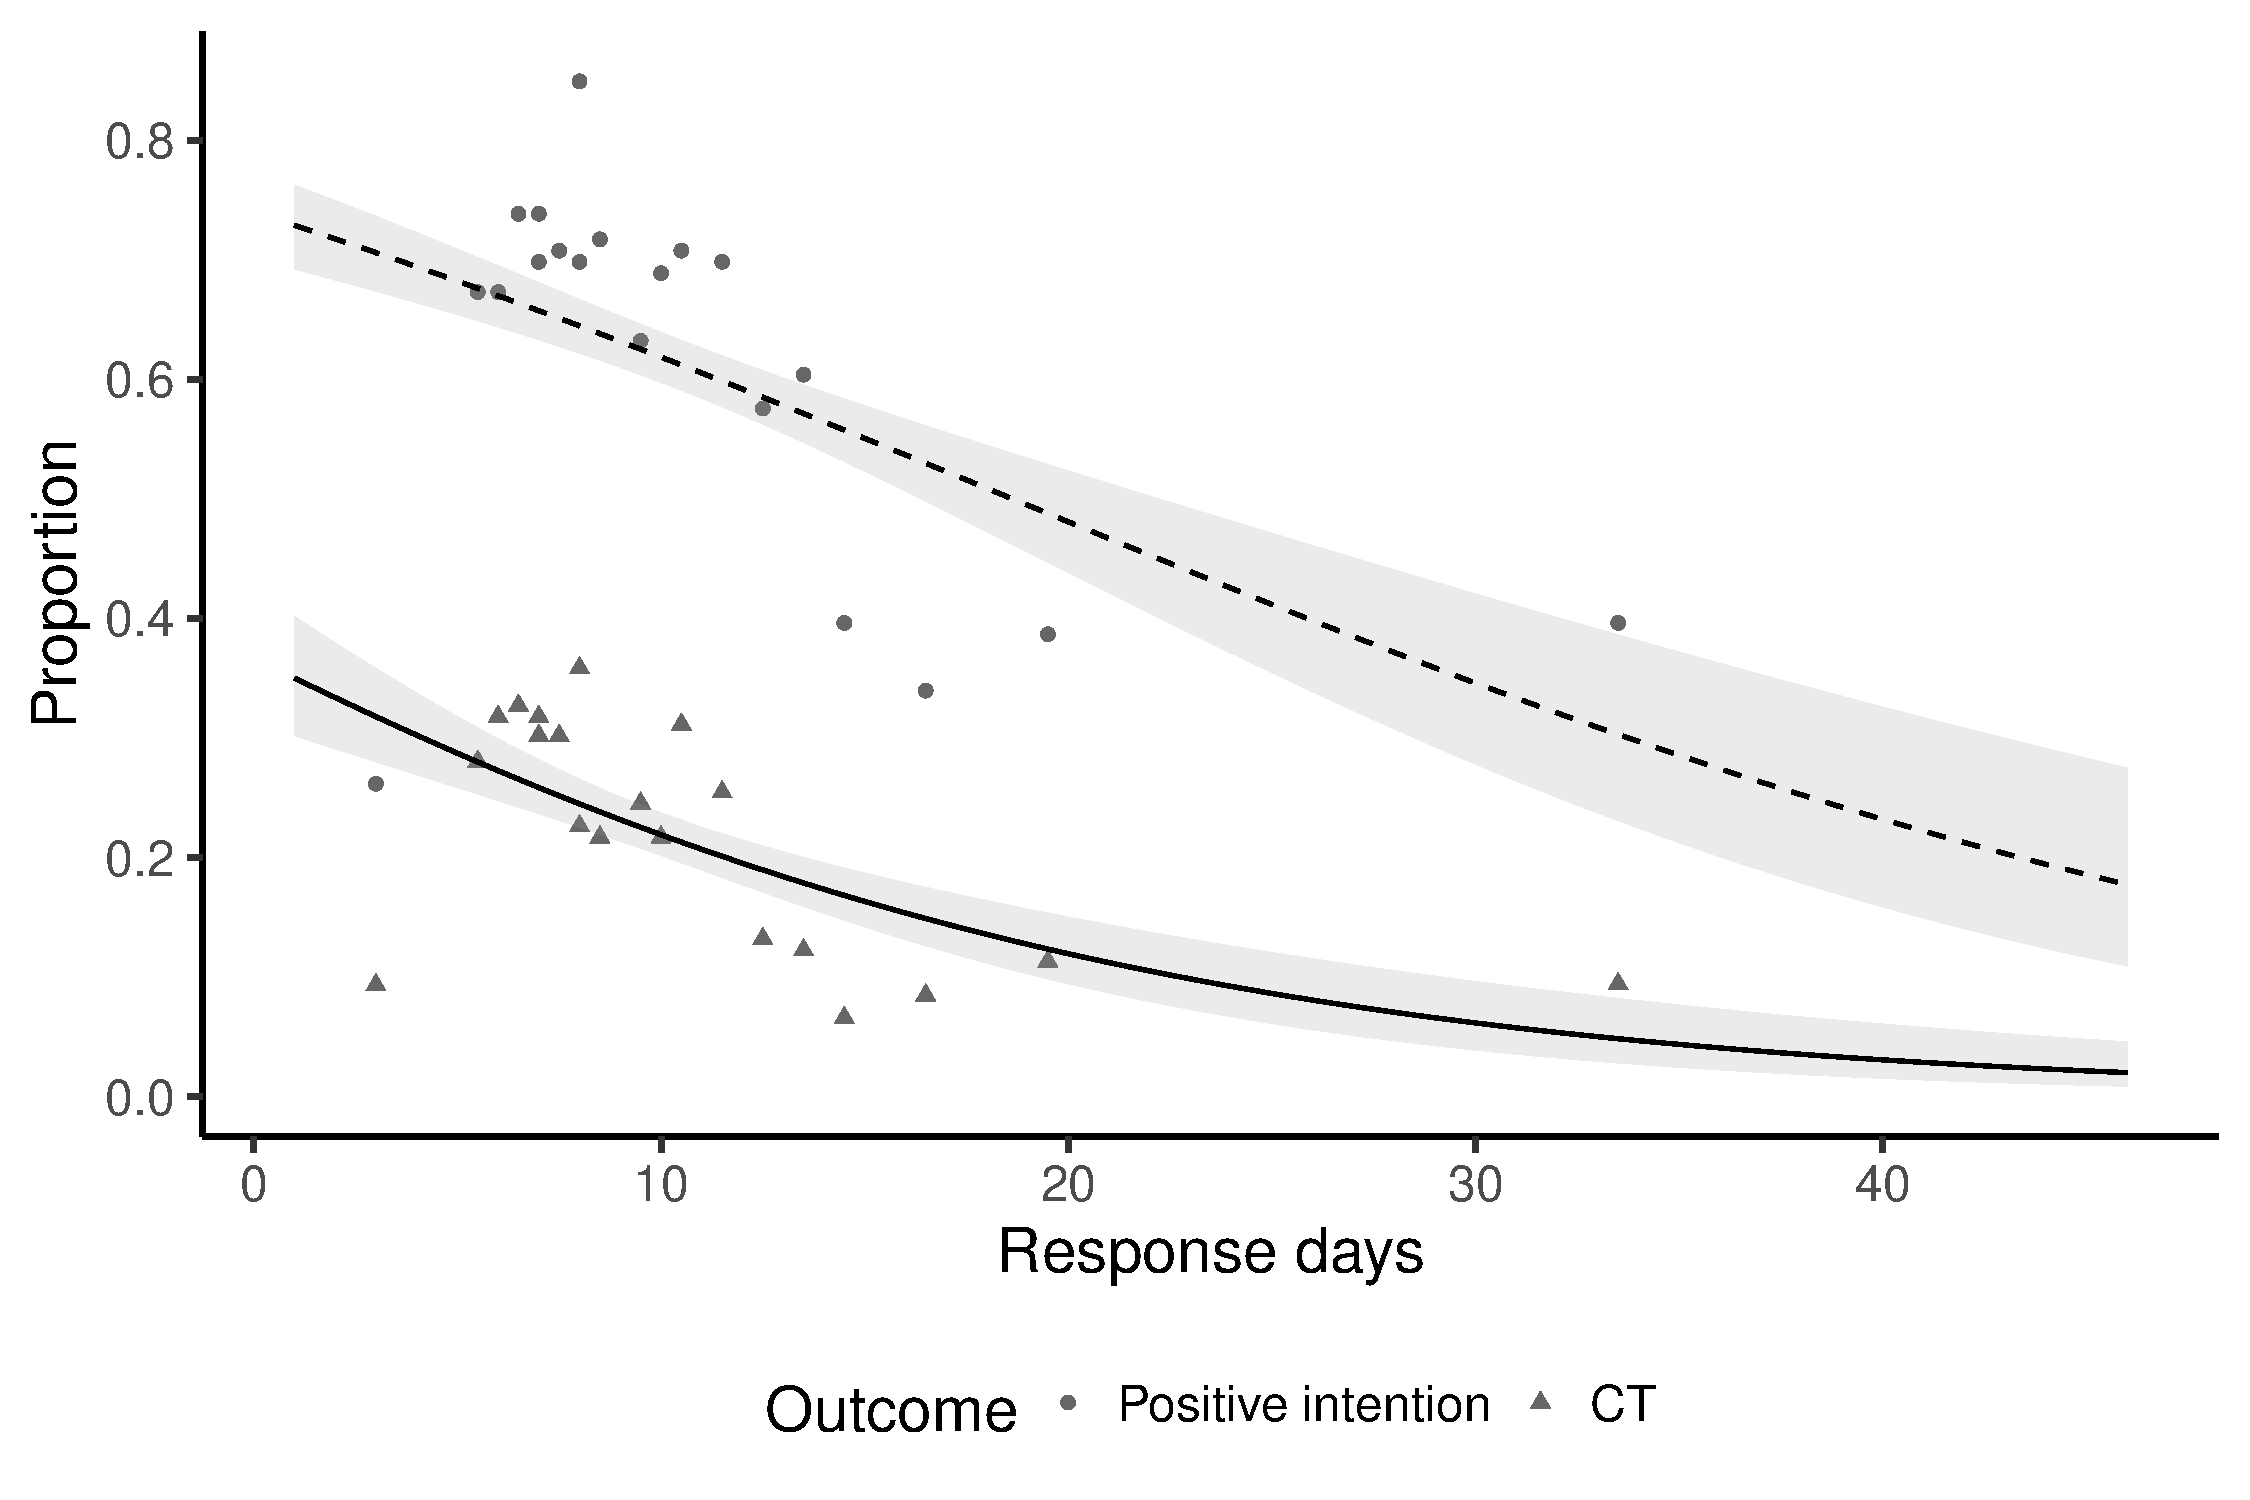
\includegraphics{JMDPRC~3/figure-latex/speed-CT-1} \caption{Binned Scatter Plot of CT (or Response with Positive Intention) vs. Response Days. \newline \emph{Note}: We run logistic regression of the CT (or response with positive intention) on response days. We excluded those who skipped the CT and used control arm. We show the regression lines and its 95 percent confidence interval.}\label{fig:speed-CT}
\end{figure}

\begin{figure}[H]
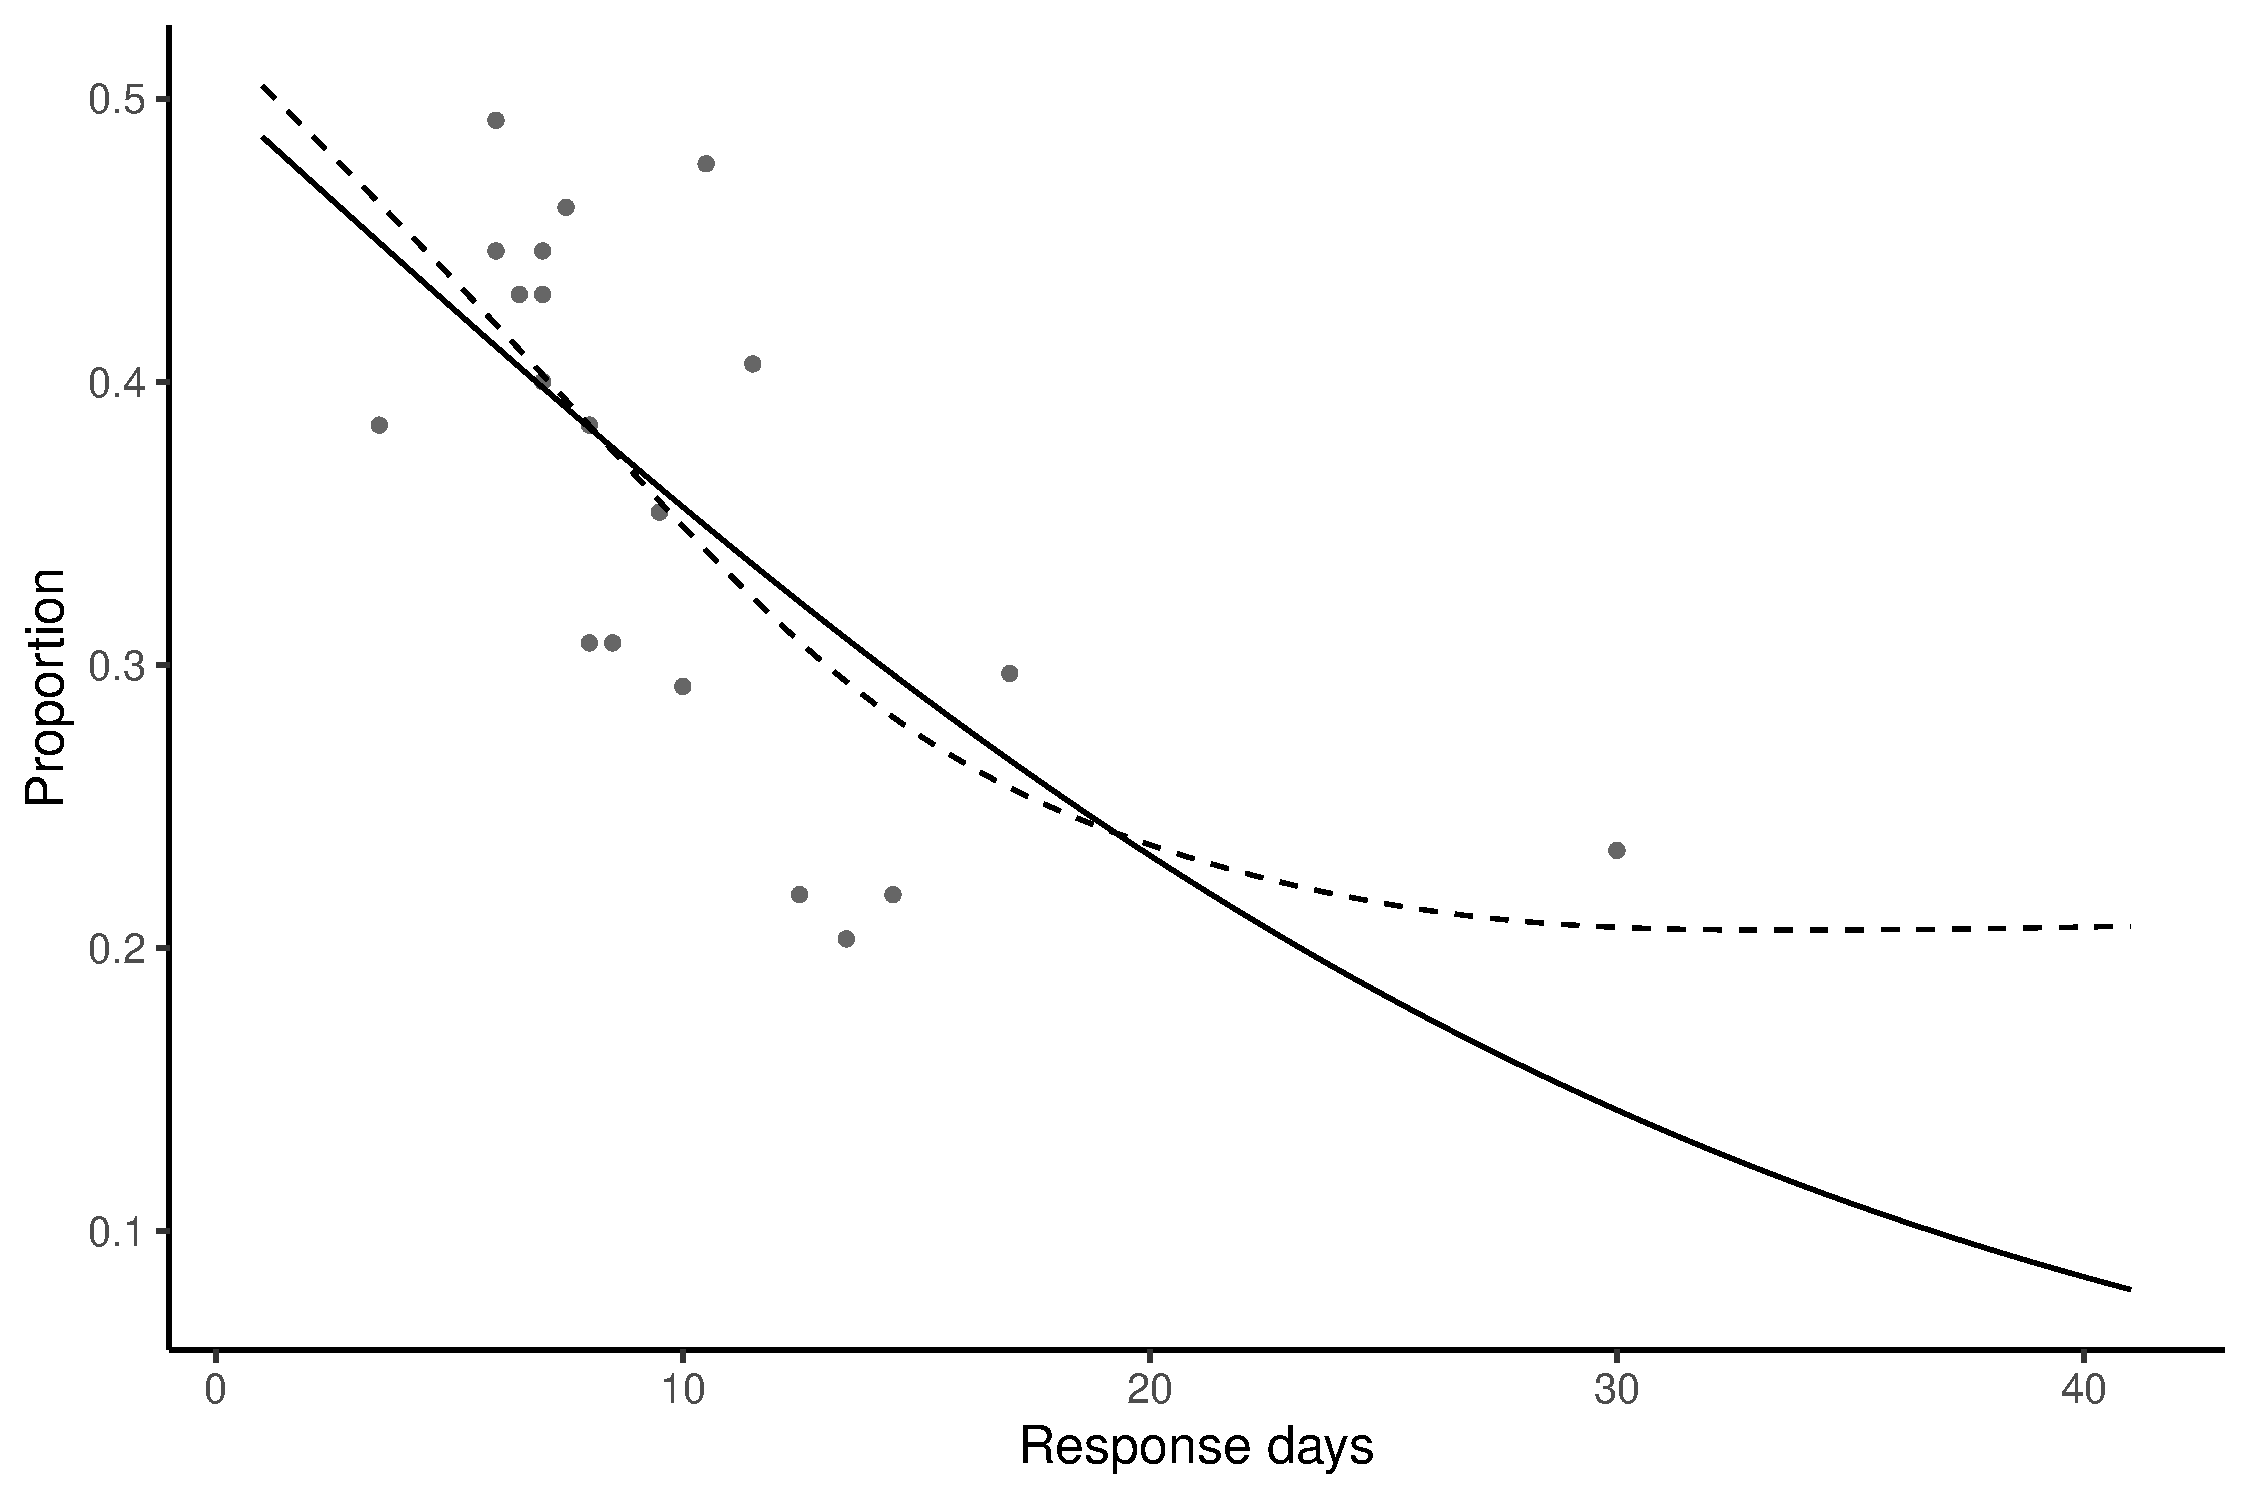
\includegraphics{JMDPRC~3/figure-latex/speed-CT-cond-response-1} \caption{Binned Scatter Plot of CT vs. Response Spped among Those Who Responded with Positive Intention. \newline \emph{Note}: We used those who responded with positive intention to donate in the control arm (experimental arm A). The dashed line represents nonparametric fitting. The solid line represents a fitted line of the logistic regression.}\label{fig:speed-CT-cond-response}
\end{figure}

\begin{figure}[t]
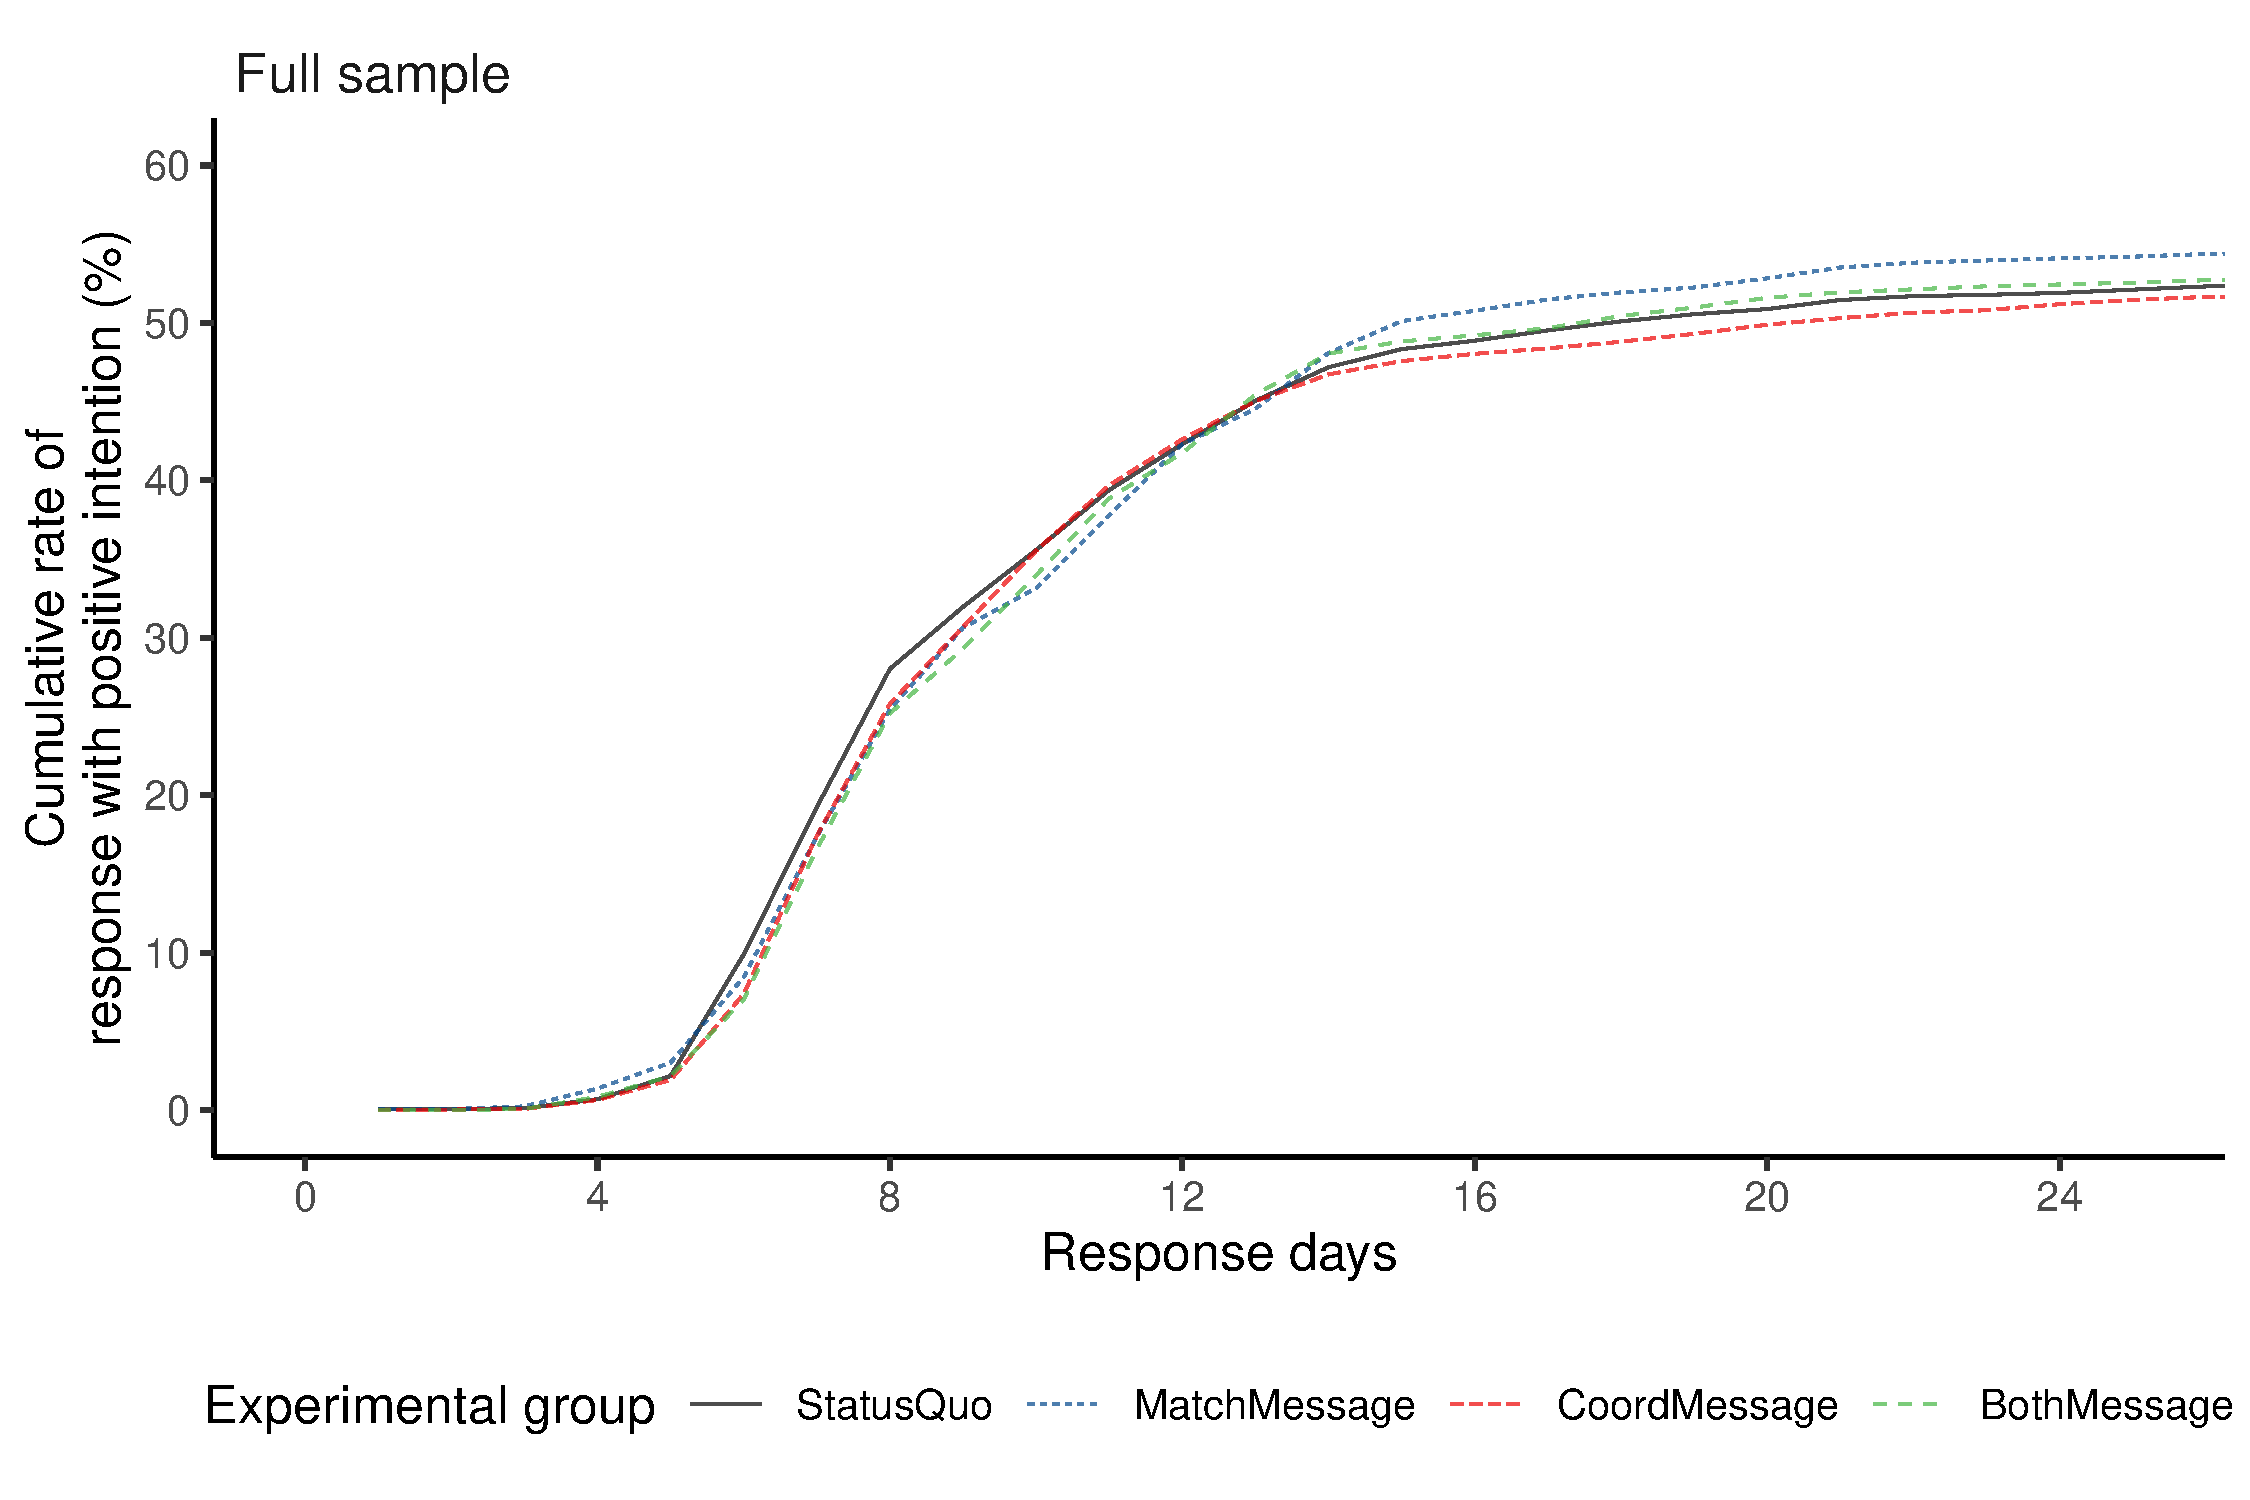
\includegraphics{JMDPRC~3/figure-latex/cumulative-response-1} \caption{Cumulative Rate of Response with Positive Intention by Treatment \newline \emph{Note}: We excluded those who skipped the CT. We only shows cumulative response rates up to 25 days after the mailing because there is no remarkable change in response rate.}\label{fig:cumulative-response}
\end{figure}

\begin{figure}[H]
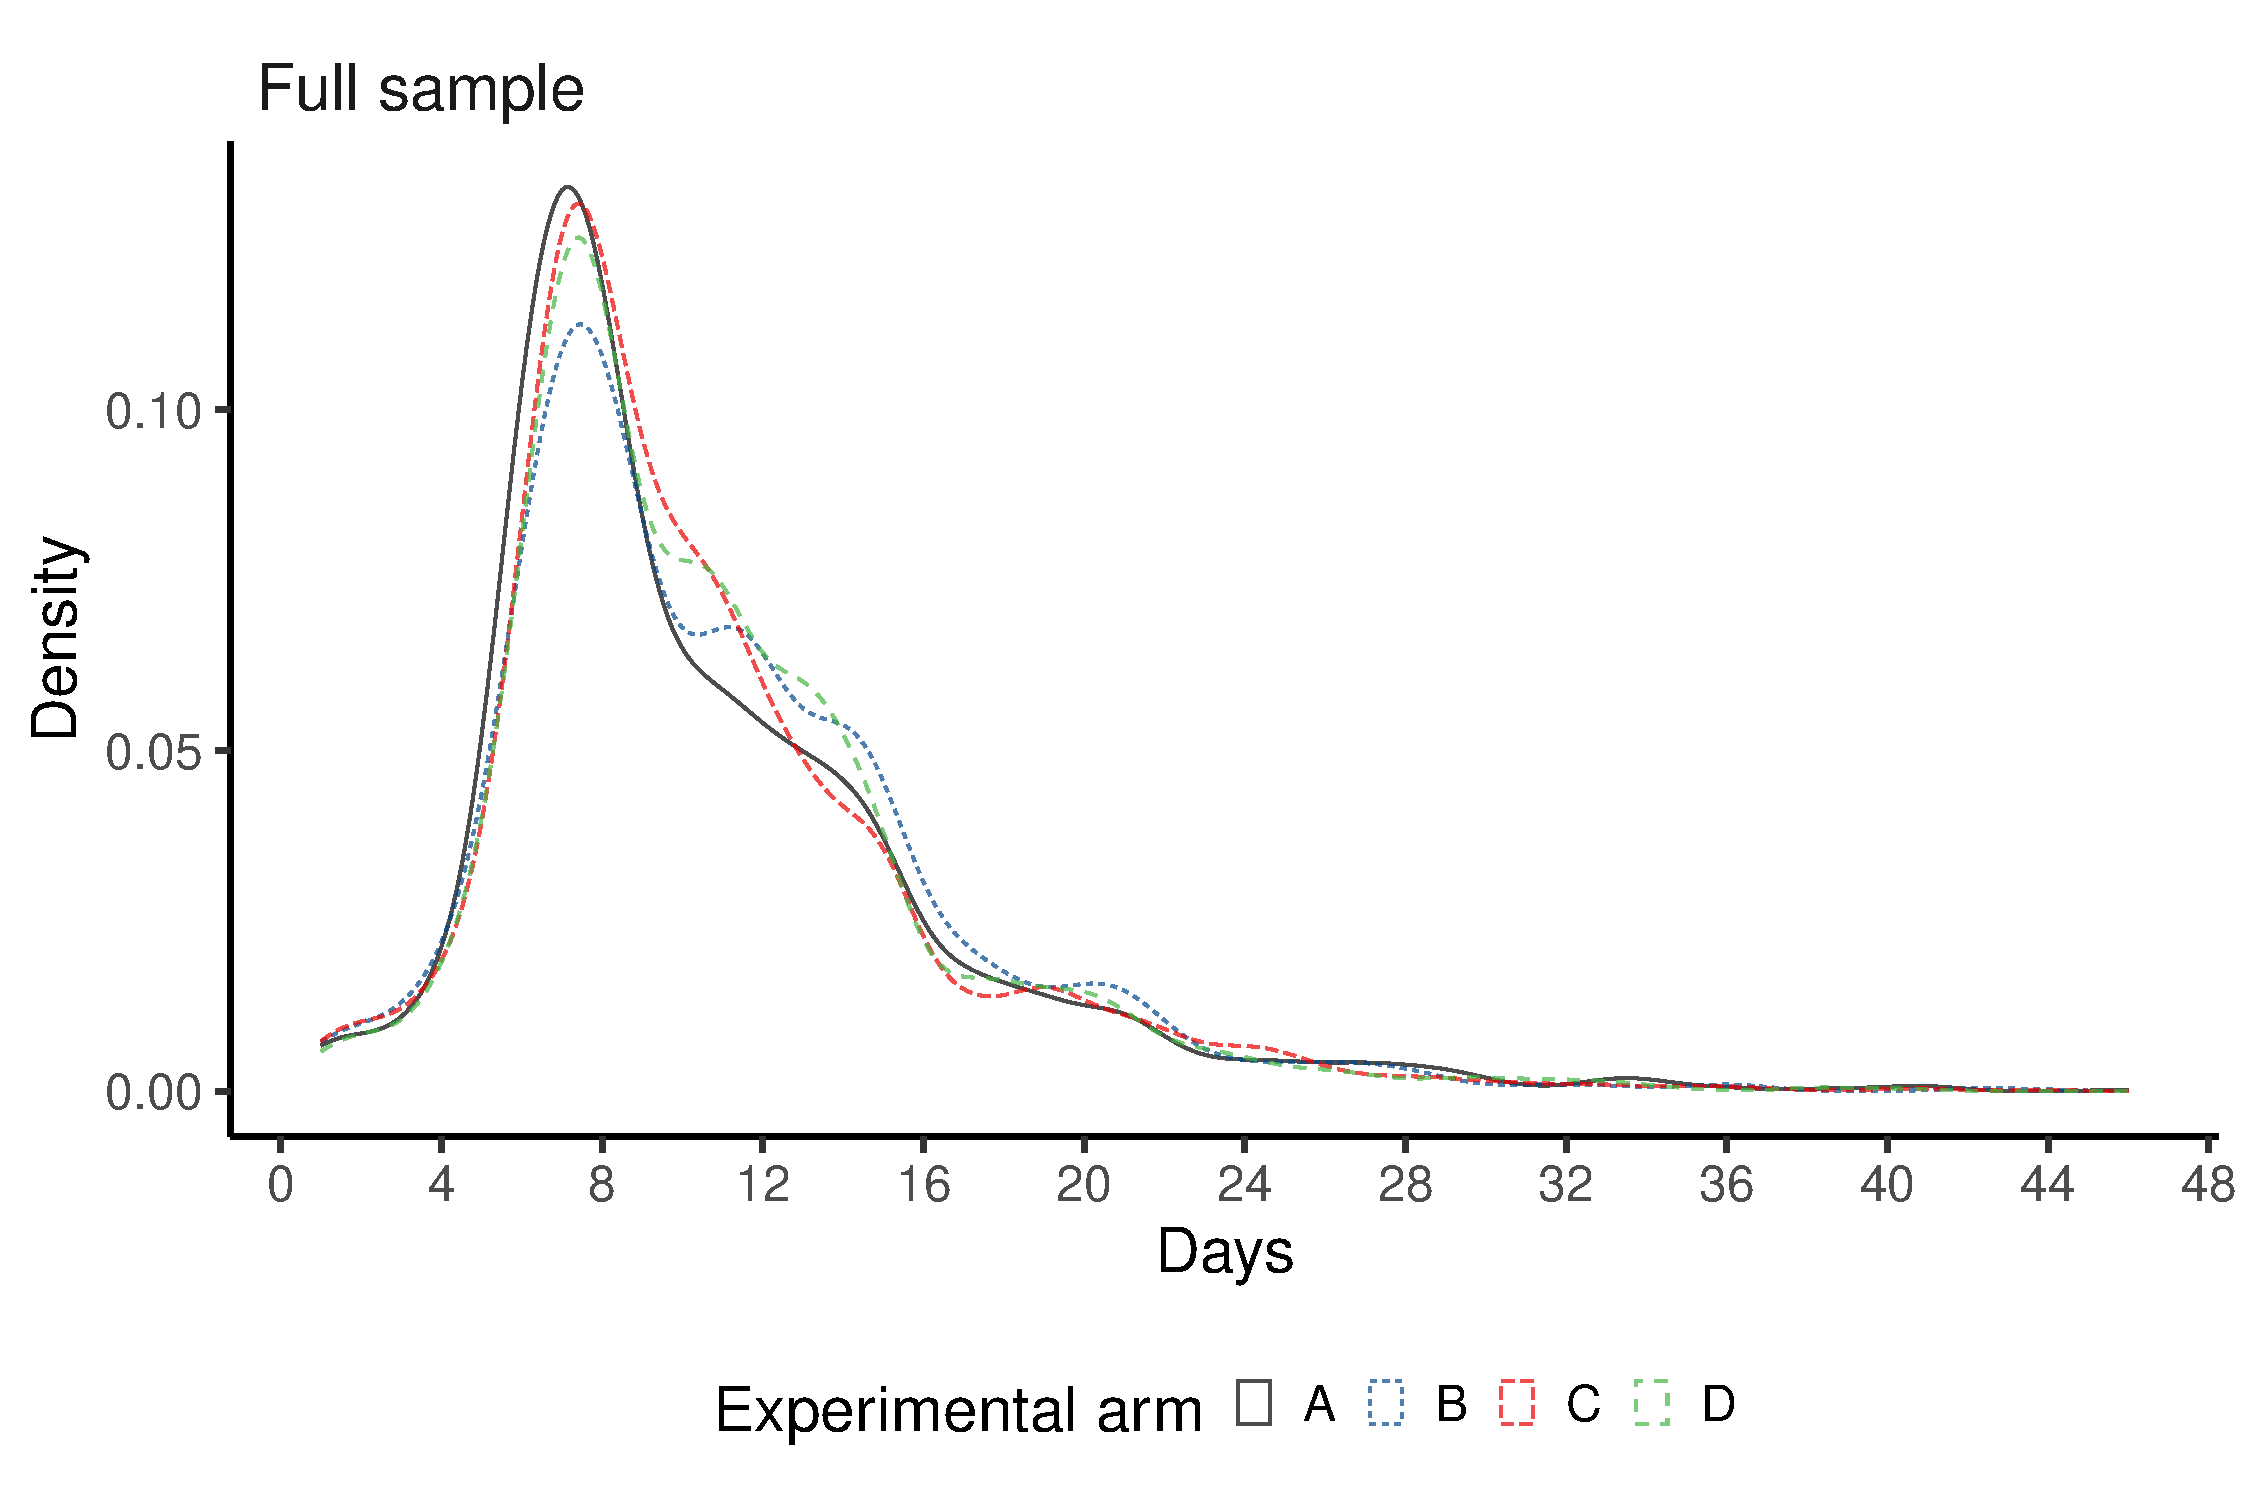
\includegraphics{JMDPRC~3/figure-latex/dist-response-speed-1} \caption{Density of Number of Days Required for Response with Positive Intention. \newline \emph{Note}: We excluded those who did not respond and skipped the CT. We also excluded those who responded after 50 days due to outliers.}\label{fig:dist-response-speed}
\end{figure}

\begin{table}[H]

\caption{\label{tab:lm-positive-time-decompose-noskip}Effect on Speed of Response with Positive Intention (Excluding Those Who Skipped the CT)}
\centering
\fontsize{8}{10}\selectfont
\begin{threeparttable}
\begin{tabular}[t]{lcccccc}
\toprule
\multicolumn{1}{c}{ } & \multicolumn{2}{c}{1--5 days} & \multicolumn{2}{c}{6--12 days} & \multicolumn{2}{c}{13--85 days} \\
\cmidrule(l{3pt}r{3pt}){2-3} \cmidrule(l{3pt}r{3pt}){4-5} \cmidrule(l{3pt}r{3pt}){6-7}
  & (1) & (2) & (3) & (4) & (5) & (6)\\
\midrule
Treatment B & \num{0.85}* & \num{0.64} & \num{-0.87} & \num{1.19} & \num{2.06}** & \num{-0.18}\\
 & (\num{0.43}) & (\num{0.46}) & (\num{1.34}) & (\num{1.48}) & (\num{0.88}) & (\num{0.94})\\
Treatment C & \num{-0.25} & \num{-0.21} & \num{0.56} & \num{1.26} & \num{-1.14} & \num{-1.07}\\
 & (\num{0.40}) & (\num{0.40}) & (\num{1.38}) & (\num{1.36}) & (\num{0.85}) & (\num{0.86})\\
Treatment D & \num{-0.02} & \num{-0.03} & \num{-0.54} & \num{-0.10} & \num{0.64} & \num{0.35}\\
 & (\num{0.41}) & (\num{0.41}) & (\num{1.38}) & (\num{1.36}) & (\num{0.89}) & (\num{0.89})\\
\midrule
Control average & 2.17 & 2.17 & 40.13 & 40.13 & 10.79 & 10.79\\
Covariates &  & X &  & X &  & X\\
Num.Obs. & \num{10547} & \num{10547} & \num{10547} & \num{10547} & \num{10547} & \num{10547}\\
\bottomrule
\end{tabular}
\begin{tablenotes}
\item \emph{Note}: * $p < 0.1$, ** $p < 0.05$, *** $p < 0.01$. The robust standard errors are in parentheses. The unit of treatment effect is a percentage point. The outcome is a dummy variable that takes a value of 1 if candidate responded with positive intention within a specified time after mailing. We excluded those who skipped the CT. Covariates are gender, age, its squared term, the number of past coordinations, the number of public holidays in the assigned week and the following week, the number of hospitals per 10 square kilometers, the number of hospitals with PBSC collection per 10 square kilometers and the number of hospitals with BM collection per 10 square kilometers. All covariates were demeaned.
\end{tablenotes}
\end{threeparttable}
\end{table}

\begin{table}[H]

\caption{\label{tab:lm-test-time-decompose-noskip}Decomposition of Effect on the CT: Response Speed Perspectives (Excluding Those Who Skipped the CT)}
\centering
\fontsize{8}{10}\selectfont
\begin{threeparttable}
\begin{tabular}[t]{lcccccc}
\toprule
\multicolumn{1}{c}{ } & \multicolumn{2}{c}{1--5 days} & \multicolumn{2}{c}{6--12 days} & \multicolumn{2}{c}{13--85 days} \\
\cmidrule(l{3pt}r{3pt}){2-3} \cmidrule(l{3pt}r{3pt}){4-5} \cmidrule(l{3pt}r{3pt}){6-7}
  & (1) & (2) & (3) & (4) & (5) & (6)\\
\midrule
Treatment B & \num{0.30} & \num{0.24} & \num{1.02} & \num{2.49}** & \num{1.27}*** & \num{0.08}\\
 & (\num{0.28}) & (\num{0.30}) & (\num{1.01}) & (\num{1.16}) & (\num{0.48}) & (\num{0.48})\\
Treatment C & \num{-0.21} & \num{-0.21} & \num{0.29} & \num{0.22} & \num{0.53} & \num{0.48}\\
 & (\num{0.25}) & (\num{0.25}) & (\num{1.03}) & (\num{1.03}) & (\num{0.47}) & (\num{0.46})\\
Treatment D & \num{0.29} & \num{0.29} & \num{0.37} & \num{0.62} & \num{0.92}* & \num{0.77}\\
 & (\num{0.29}) & (\num{0.29}) & (\num{1.03}) & (\num{1.03}) & (\num{0.48}) & (\num{0.48})\\
\midrule
Control average & 0.90 & 0.90 & 15.68 & 15.68 & 2.54 & 2.54\\
Covariates &  & X &  & X &  & X\\
Num.Obs. & \num{10547} & \num{10547} & \num{10547} & \num{10547} & \num{10547} & \num{10547}\\
\bottomrule
\end{tabular}
\begin{tablenotes}
\item \emph{Note}: * $p < 0.1$, ** $p < 0.05$, *** $p < 0.01$. The robust standard errors are in parentheses. The unit of treatment effect is a percentage point. The outcome is a dummy variable that takes a value of 1 if candidate responded with positive intention within a specified time after mailing and reached the CT. Covariates are gender, age, its squared term, the number of past coordinations, the number of public holidays in the assigned week and the following week, the number of hospitals per 10 square kilometers, the number of hospitals with PBSC collection per 10 square kilometers and the number of hospitals with BM collection per 10 square kilometers. All covariates were demeaned.
\end{tablenotes}
\end{threeparttable}
\end{table}

\begin{figure}[H]
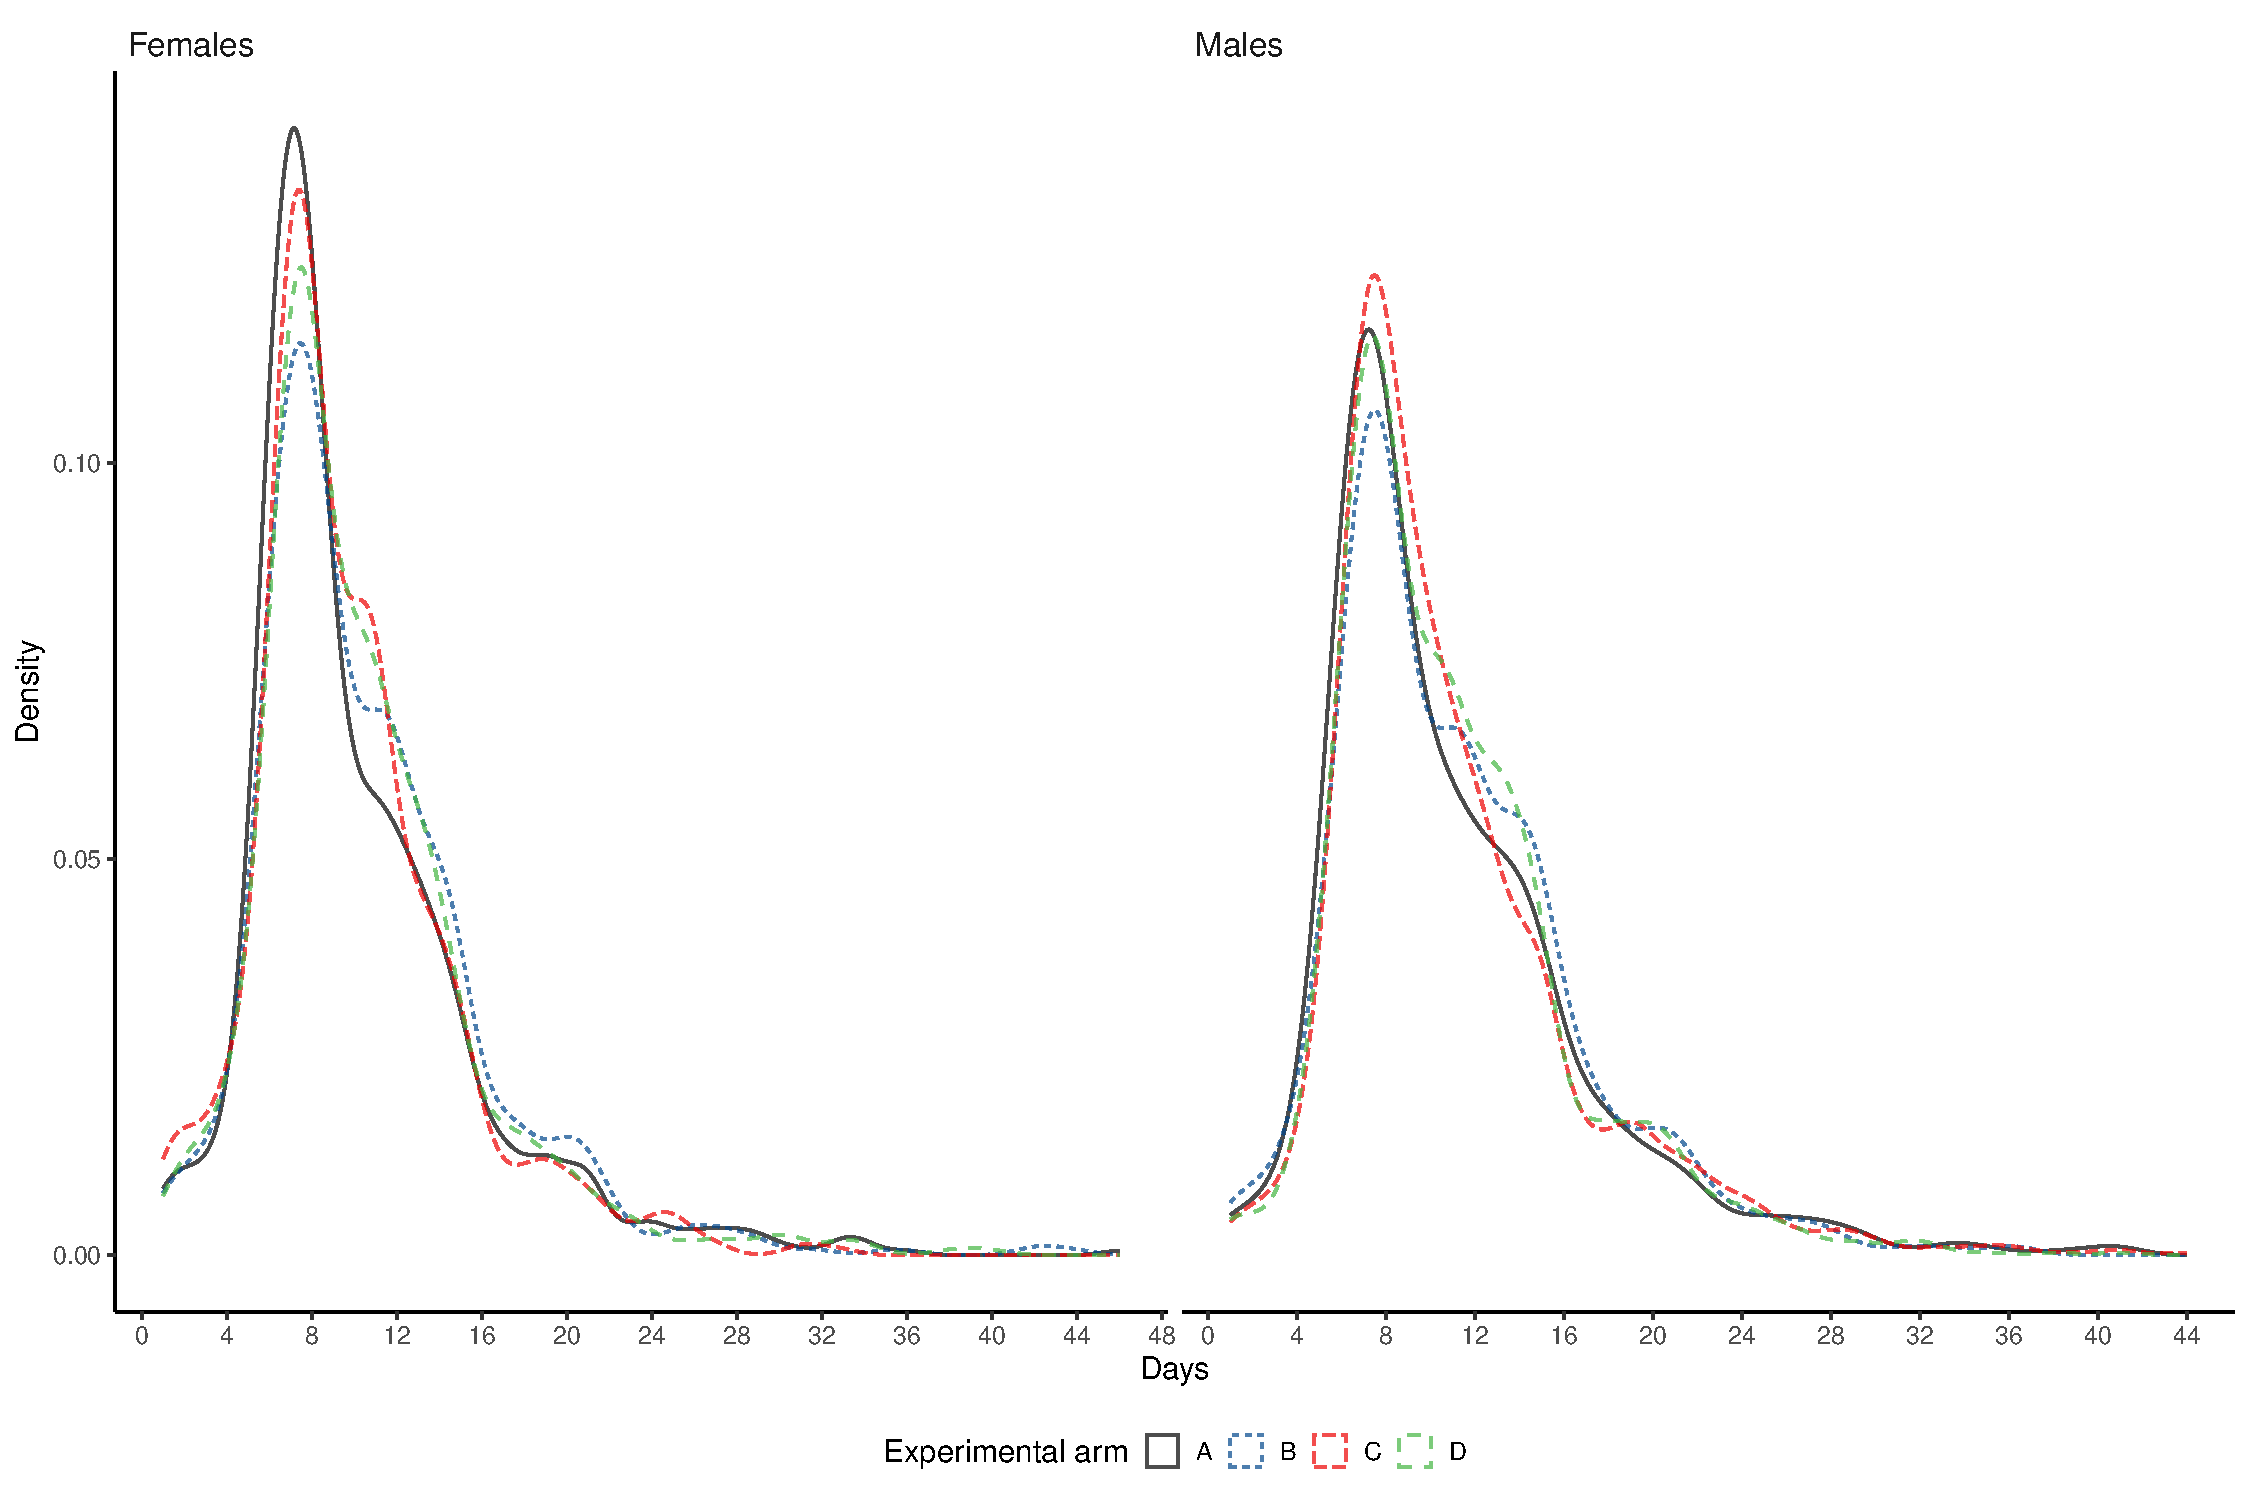
\includegraphics{JMDPRC~3/figure-latex/dist-response-speed-by-gender-1} \caption{Density of Number of Days Required for Response with Positive Intention by Gender. \newline \emph{Note}: We excluded those who did not respond and skipped the CT. We also excluded those who responded after 50 days due to outliers.}\label{fig:dist-response-speed-by-gender}
\end{figure}

\begin{table}[H]

\caption{\label{tab:lm-interaction-gender-int-time-decompose-noskip}Heterogenity of Effect on Speed of Response with Positive Intention by Gender (Excluding Those Who Skipped the CT)}
\centering
\fontsize{8}{10}\selectfont
\begin{threeparttable}
\begin{tabular}[t]{lcccccc}
\toprule
\multicolumn{1}{c}{ } & \multicolumn{2}{c}{1--5 days} & \multicolumn{2}{c}{6--12 days} & \multicolumn{2}{c}{13--85 days} \\
\cmidrule(l{3pt}r{3pt}){2-3} \cmidrule(l{3pt}r{3pt}){4-5} \cmidrule(l{3pt}r{3pt}){6-7}
  & (1) & (2) & (3) & (4) & (5) & (6)\\
\midrule
Treatment B & \num{-0.30} & \num{-0.16} & \num{-2.61} & \num{-1.08} & \num{2.14} & \num{0.31}\\
 & (\num{0.71}) & (\num{0.78}) & (\num{2.20}) & (\num{2.42}) & (\num{1.37}) & (\num{1.45})\\
Treatment C & \num{-0.68} & \num{-0.80} & \num{-0.07} & \num{0.14} & \num{-0.62} & \num{-0.44}\\
 & (\num{0.71}) & (\num{0.71}) & (\num{2.28}) & (\num{2.27}) & (\num{1.34}) & (\num{1.34})\\
Treatment D & \num{-1.11}* & \num{-1.10} & \num{-2.44} & \num{-2.26} & \num{1.45} & \num{1.20}\\
 & (\num{0.67}) & (\num{0.67}) & (\num{2.23}) & (\num{2.22}) & (\num{1.38}) & (\num{1.38})\\
Male & \num{-0.97} & \num{-0.87} & \num{-5.37}*** & \num{-6.24}*** & \num{1.93} & \num{2.45}*\\
 & (\num{0.64}) & (\num{0.74}) & (\num{2.05}) & (\num{2.35}) & (\num{1.27}) & (\num{1.49})\\
Treatment B $\times$ Male & \num{1.85}** & \num{1.26} & \num{2.87} & \num{3.50} & \num{-0.16} & \num{-0.74}\\
 & (\num{0.90}) & (\num{0.97}) & (\num{2.78}) & (\num{3.06}) & (\num{1.79}) & (\num{1.90})\\
Treatment C $\times$ Male & \num{0.71} & \num{0.98} & \num{1.14} & \num{1.73} & \num{-0.87} & \num{-0.97}\\
 & (\num{0.85}) & (\num{0.85}) & (\num{2.87}) & (\num{2.84}) & (\num{1.74}) & (\num{1.74})\\
Treatment D $\times$ Male & \num{1.78}** & \num{1.77}** & \num{3.05} & \num{3.45} & \num{-1.32} & \num{-1.36}\\
 & (\num{0.85}) & (\num{0.85}) & (\num{2.84}) & (\num{2.81}) & (\num{1.80}) & (\num{1.80})\\
\midrule
Covariates &  & X &  & X &  & X\\
Num.Obs. & \num{10547} & \num{10547} & \num{10547} & \num{10547} & \num{10547} & \num{10547}\\
\bottomrule
\end{tabular}
\begin{tablenotes}
\item \emph{Note}: * $p < 0.1$, ** $p < 0.05$, *** $p < 0.01$. The robust standard errors are in parentheses. The unit of treatment effect is a percentage point. The outcome is a dummy variable that takes a value of 1 if candidate responded with positive intention within a specified time after mailing. We excluded those who skipped the CT. Covariates are age, its squared term, the number of past coordinations, the number of public holidays in the assigned week and the following week, the number of hospitals per 10 square kilometers, the number of hospitals with PBSC collection per 10 square kilometers and the number of hospitals with BM collection per 10 square kilometers. All covariates were demeaned. We also controlled cross term of each covariate and gender dummy.
\end{tablenotes}
\end{threeparttable}
\end{table}

\begin{table}[H]

\caption{\label{tab:lh-interaction-gender-int-time-decompose-noskip}Effect on Speed of Response with Positive Intention for Specific Gender Group (Excluding Those Who Skipped the CT)}
\centering
\fontsize{8}{10}\selectfont
\begin{threeparttable}
\begin{tabular}[t]{llcccccc}
\toprule
\multicolumn{2}{c}{ } & \multicolumn{2}{c}{1--5 days} & \multicolumn{2}{c}{6--12 days} & \multicolumn{2}{c}{13--85 days} \\
\cmidrule(l{3pt}r{3pt}){3-4} \cmidrule(l{3pt}r{3pt}){5-6} \cmidrule(l{3pt}r{3pt}){7-8}
Group & Treatment & (1) & (2) & (3) & (4) & (5) & (6)\\
\midrule
Female & B & -0.30 (0.71) & -0.16 (0.78) & -2.61 (2.20) & -1.08 (2.42) & 2.14 (1.37) & 0.31 (1.45)\\
 & C & -0.68 (0.71) & -0.80 (0.71) & -0.07 (2.28) & 0.14 (2.27) & -0.62 (1.34) & -0.44 (1.34)\\
 & D & -1.11 (0.67)* & -1.10 (0.67) & -2.44 (2.23) & -2.26 (2.22) & 1.45 (1.38) & 1.20 (1.38)\\
Male & B & 1.55 (0.54)*** & 1.10 (0.57)* & 0.26 (1.69) & 2.42 (1.87) & 1.98 (1.15)* & -0.43 (1.23)\\
 & C & 0.03 (0.48) & 0.18 (0.48) & 1.07 (1.74) & 1.86 (1.70) & -1.49 (1.11) & -1.41 (1.11)\\
 & D & 0.67 (0.52) & 0.67 (0.52) & 0.61 (1.75) & 1.18 (1.72) & 0.13 (1.16) & -0.16 (1.16)\\
\midrule
 & Covariates &  & X &  & X &  & X\\
\bottomrule
\end{tabular}
\begin{tablenotes}
\item \emph{Note}: * $p < 0.1$, ** $p < 0.05$, *** $p < 0.01$. The robust standard errors are in parentheses. We performed a linear combination test on the coefficients of the linear probability model presented in Table \ref{tab:lm-interaction-gender-int-time-decompose-noskip}. The null hypothesis for females is that the treatment dummy is zero. The null hypothesis for males is that the sum of the treatment dummy and the cross term of the treatment dummy and the gender dummy is zero.
\end{tablenotes}
\end{threeparttable}
\end{table}

\begin{figure}[H]
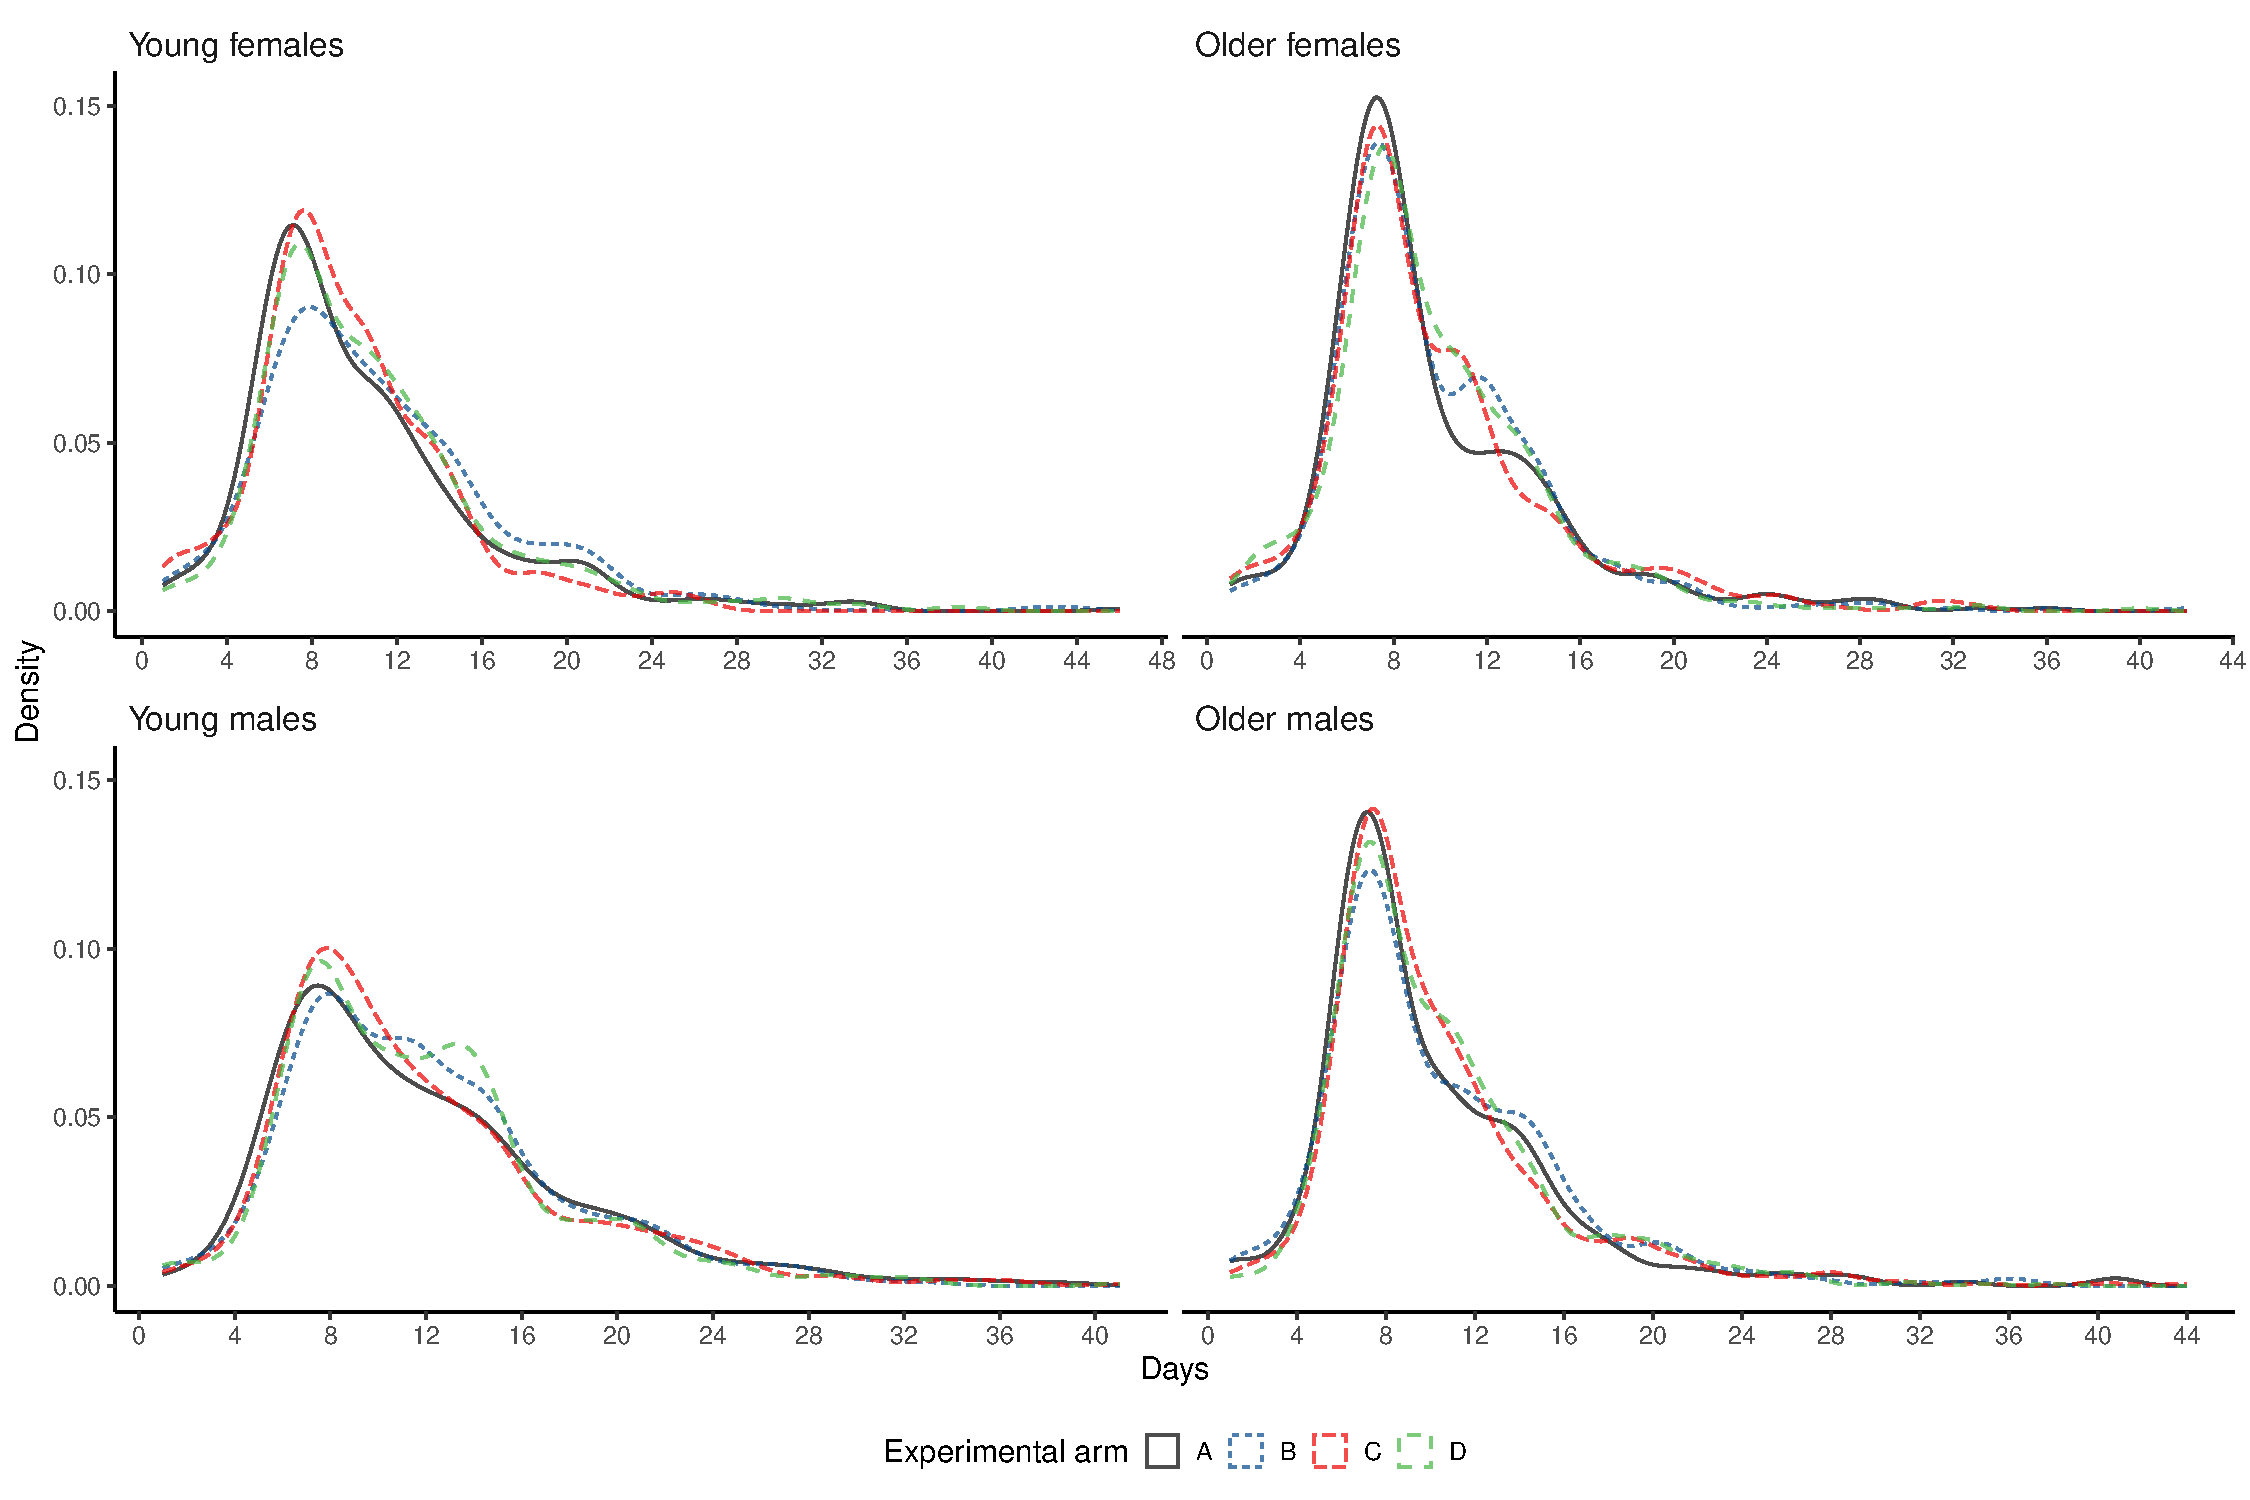
\includegraphics{JMDPRC~3/figure-latex/dist-response-speed-by-gender-age-1} \caption{Density of Number of Days Required for Response with Positive Intention by Gender. \newline \emph{Note}: We excluded those who did not respond and skipped the CT. We also excluded those who responded after 50 days due to outliers.}\label{fig:dist-response-speed-by-gender-age}
\end{figure}

\begin{table}[H]

\caption{\label{tab:lm-interaction-gender-age-int-time-decompose-noskip}Heterogenity of Effect on Speed of Response with Positive Intention by Gender and Age (Excluding Those Who Skipped the CT)}
\centering
\fontsize{8}{10}\selectfont
\begin{threeparttable}
\begin{tabular}[t]{lcccccc}
\toprule
\multicolumn{1}{c}{ } & \multicolumn{2}{c}{1--5 days} & \multicolumn{2}{c}{6--12 days} & \multicolumn{2}{c}{13--85 days} \\
\cmidrule(l{3pt}r{3pt}){2-3} \cmidrule(l{3pt}r{3pt}){4-5} \cmidrule(l{3pt}r{3pt}){6-7}
  & (1) & (2) & (3) & (4) & (5) & (6)\\
\midrule
Treatment B & \num{-0.20} & \num{0.19} & \num{-5.14}* & \num{-4.13} & \num{2.79} & \num{2.03}\\
 & (\num{1.02}) & (\num{1.10}) & (\num{2.97}) & (\num{3.28}) & (\num{1.91}) & (\num{2.03})\\
Treatment C & \num{-1.45} & \num{-1.71}* & \num{-0.62} & \num{-1.24} & \num{-0.99} & \num{-0.88}\\
 & (\num{0.92}) & (\num{0.91}) & (\num{3.05}) & (\num{3.05}) & (\num{1.80}) & (\num{1.80})\\
Treatment D & \num{-1.44} & \num{-1.43} & \num{-4.50} & \num{-4.40} & \num{0.75} & \num{0.71}\\
 & (\num{0.93}) & (\num{0.92}) & (\num{3.03}) & (\num{3.03}) & (\num{1.88}) & (\num{1.89})\\
Older female & \num{-0.29} & \num{-0.23} & \num{8.33}** & \num{8.06}** & \num{0.04} & \num{0.95}\\
 & (\num{1.07}) & (\num{1.10}) & (\num{3.23}) & (\num{3.32}) & (\num{1.93}) & (\num{1.99})\\
Young male & \num{-1.78}** & \num{-1.61}* & \num{-9.75}*** & \num{-9.73}*** & \num{2.67} & \num{2.89}\\
 & (\num{0.87}) & (\num{0.89}) & (\num{2.82}) & (\num{2.90}) & (\num{1.83}) & (\num{1.87})\\
Older male & \num{-0.54} & \num{-0.28} & \num{6.11}** & \num{5.54}* & \num{1.32} & \num{2.50}\\
 & (\num{0.94}) & (\num{0.97}) & (\num{2.85}) & (\num{2.94}) & (\num{1.74}) & (\num{1.79})\\
Treatment B $\times$ Older female & \num{-0.22} & \num{-0.83} & \num{6.04} & \num{6.83} & \num{-1.42} & \num{-3.54}\\
 & (\num{1.43}) & (\num{1.56}) & (\num{4.39}) & (\num{4.86}) & (\num{2.74}) & (\num{2.88})\\
Treatment C $\times$ Older female & \num{1.76} & \num{1.98} & \num{2.43} & \num{3.00} & \num{0.88} & \num{0.91}\\
 & (\num{1.45}) & (\num{1.44}) & (\num{4.57}) & (\num{4.57}) & (\num{2.69}) & (\num{2.69})\\
Treatment D $\times$ Older female & \num{0.69} & \num{0.67} & \num{4.72} & \num{4.73} & \num{1.50} & \num{1.28}\\
 & (\num{1.34}) & (\num{1.34}) & (\num{4.46}) & (\num{4.46}) & (\num{2.76}) & (\num{2.77})\\
Treatment B $\times$ Young male & \num{1.42} & \num{0.72} & \num{7.80}** & \num{8.28}** & \num{-1.48} & \num{-1.98}\\
 & (\num{1.21}) & (\num{1.30}) & (\num{3.77}) & (\num{4.19}) & (\num{2.55}) & (\num{2.75})\\
Treatment C $\times$ Young male & \num{1.79}* & \num{2.10}* & \num{1.07} & \num{1.58} & \num{-0.02} & \num{-0.01}\\
 & (\num{1.09}) & (\num{1.07}) & (\num{3.83}) & (\num{3.83}) & (\num{2.43}) & (\num{2.43})\\
Treatment D $\times$ Young male & \num{1.32} & \num{1.29} & \num{5.07} & \num{4.99} & \num{-1.41} & \num{-1.52}\\
 & (\num{1.07}) & (\num{1.06}) & (\num{3.85}) & (\num{3.86}) & (\num{2.52}) & (\num{2.53})\\
Treatment B $\times$ Older male & \num{2.13} & \num{1.13} & \num{3.78} & \num{5.75} & \num{-0.24} & \num{-2.94}\\
 & (\num{1.33}) & (\num{1.42}) & (\num{3.82}) & (\num{4.25}) & (\num{2.47}) & (\num{2.60})\\
Treatment C $\times$ Older male & \num{1.30} & \num{1.68} & \num{4.74} & \num{5.45} & \num{-1.25} & \num{-1.26}\\
 & (\num{1.20}) & (\num{1.18}) & (\num{3.97}) & (\num{3.97}) & (\num{2.35}) & (\num{2.35})\\
Treatment D $\times$ Older male & \num{2.97}** & \num{2.98}** & \num{6.11} & \num{6.54}* & \num{0.09} & \num{-0.29}\\
 & (\num{1.28}) & (\num{1.27}) & (\num{3.93}) & (\num{3.94}) & (\num{2.46}) & (\num{2.48})\\
\midrule
Covariates &  & X &  & X &  & X\\
Num.Obs. & \num{10547} & \num{10547} & \num{10547} & \num{10547} & \num{10547} & \num{10547}\\
\bottomrule
\end{tabular}
\begin{tablenotes}
\item \emph{Note}: * $p < 0.1$, ** $p < 0.05$, *** $p < 0.01$. The robust standard errors are in parentheses. The unit of treatment effect is a percentage point. The outcome is a dummy variable that takes a value of 1 if candidate responded with positive intention within a specified time after mailing. We excluded those who skipped the CT. We created two age groups (Younger/Older) based on age 40. Covariates are age, its squared term, the number of past coordinations, the number of public holidays in the assigned week and the following week, the number of hospitals per 10 square kilometers, the number of hospitals with PBSC collection per 10 square kilometers and the number of hospitals with BM collection per 10 square kilometers. All covariates were demeaned. We also controlled cross term of each covariate and gender-age group dummies.
\end{tablenotes}
\end{threeparttable}
\end{table}

\begin{table}[H]

\caption{\label{tab:lh-interaction-gender-age-int-time-decompose-noskip}Effect on Speed of Response with Positive Intention for Specific Gender-Age Group (Excluding Those Who Skipped the CT)}
\centering
\fontsize{8}{10}\selectfont
\begin{threeparttable}
\begin{tabular}[t]{llcccccc}
\toprule
\multicolumn{2}{c}{ } & \multicolumn{2}{c}{1--5 days} & \multicolumn{2}{c}{6--12 days} & \multicolumn{2}{c}{13--85 days} \\
\cmidrule(l{3pt}r{3pt}){3-4} \cmidrule(l{3pt}r{3pt}){5-6} \cmidrule(l{3pt}r{3pt}){7-8}
Group & Treatment & (1) & (2) & (3) & (4) & (5) & (6)\\
\midrule
Young female & B & -0.20 (1.02) & 0.19 (1.10) & -5.14 (2.97)* & -4.13 (3.28) & 2.79 (1.91) & 2.03 (2.03)\\
 & C & -1.45 (0.92) & -1.71 (0.91)* & -0.62 (3.05) & -1.24 (3.05) & -0.99 (1.80) & -0.88 (1.80)\\
 & D & -1.44 (0.93) & -1.43 (0.92) & -4.50 (3.03) & -4.40 (3.03) & 0.75 (1.88) & 0.71 (1.89)\\
Older female & B & -0.43 (1.00) & -0.64 (1.11) & 0.90 (3.24) & 2.70 (3.59) & 1.37 (1.97) & -1.51 (2.05)\\
 & C & 0.30 (1.12) & 0.27 (1.12) & 1.81 (3.40) & 1.76 (3.40) & -0.12 (2.00) & 0.03 (1.99)\\
 & D & -0.75 (0.97) & -0.76 (0.98) & 0.21 (3.27) & 0.34 (3.27) & 2.25 (2.02) & 2.00 (2.03)\\
Young male & B & 1.21 (0.65)* & 0.91 (0.69) & 2.66 (2.33) & 4.16 (2.60) & 1.31 (1.69) & 0.04 (1.85)\\
 & C & 0.34 (0.57) & 0.38 (0.57) & 0.45 (2.32) & 0.34 (2.32) & -1.01 (1.63) & -0.89 (1.63)\\
 & D & -0.12 (0.54) & -0.14 (0.53) & 0.56 (2.38) & 0.59 (2.38) & -0.66 (1.69) & -0.80 (1.69)\\
Older male & B & 1.92 (0.86)** & 1.32 (0.89) & -1.36 (2.40) & 1.62 (2.71) & 2.55 (1.57) & -0.91 (1.63)\\
 & C & -0.15 (0.76) & -0.03 (0.76) & 4.12 (2.53) & 4.21 (2.53)* & -2.24 (1.50) & -2.14 (1.50)\\
 & D & 1.53 (0.88)* & 1.55 (0.88)* & 1.61 (2.50) & 2.15 (2.51) & 0.84 (1.59) & 0.43 (1.60)\\
\midrule
 & Covariates &  & X &  & X &  & X\\
\bottomrule
\end{tabular}
\begin{tablenotes}
\item \emph{Note}: * $p < 0.1$, ** $p < 0.05$, *** $p < 0.01$. The robust standard errors are in parentheses. We performed a linear combination test on the coefficients of the linear probability model presented in Table \ref{tab:lm-interaction-gender-age-int-time-decompose-noskip}. The null hypothesis for young women is that the treatment dummy is zero. The null hypothesis for the other gender-age groups is that the sum of the treatment dummy and the cross term of the treatment dummy and the gender-age group dummy is zero.
\end{tablenotes}
\end{threeparttable}
\end{table}

\begin{table}[H]

\caption{\label{tab:lm-interaction-gender-test-time-decompose-noskip}Heterogeneity of Decomposition of Effect on the CT: Response Speed Perspectives (Excluding Those Who Skipped the CT)}
\centering
\fontsize{8}{10}\selectfont
\begin{threeparttable}
\begin{tabular}[t]{lcccccc}
\toprule
\multicolumn{1}{c}{ } & \multicolumn{2}{c}{1--5 days} & \multicolumn{2}{c}{6--12 days} & \multicolumn{2}{c}{13--85 days} \\
\cmidrule(l{3pt}r{3pt}){2-3} \cmidrule(l{3pt}r{3pt}){4-5} \cmidrule(l{3pt}r{3pt}){6-7}
  & (1) & (2) & (3) & (4) & (5) & (6)\\
\midrule
Treatment B & \num{-0.41} & \num{-0.55} & \num{0.70} & \num{1.30} & \num{1.69}*** & \num{0.99}*\\
 & (\num{0.39}) & (\num{0.40}) & (\num{1.64}) & (\num{1.83}) & (\num{0.60}) & (\num{0.59})\\
Treatment C & \num{-0.65}* & \num{-0.64}* & \num{-1.27} & \num{-1.50} & \num{1.02}* & \num{1.04}*\\
 & (\num{0.37}) & (\num{0.37}) & (\num{1.65}) & (\num{1.66}) & (\num{0.57}) & (\num{0.57})\\
Treatment D & \num{-0.18} & \num{-0.19} & \num{0.73} & \num{0.82} & \num{2.26}*** & \num{2.16}***\\
 & (\num{0.42}) & (\num{0.42}) & (\num{1.67}) & (\num{1.67}) & (\num{0.65}) & (\num{0.66})\\
Male & \num{-0.09} & \num{0.11} & \num{-0.37} & \num{0.34} & \num{2.40}*** & \num{2.75}***\\
 & (\num{0.40}) & (\num{0.45}) & (\num{1.52}) & (\num{1.77}) & (\num{0.58}) & (\num{0.73})\\
Treatment B $\times$ Male & \num{1.14}** & \num{1.32}** & \num{0.51} & \num{1.88} & \num{-0.70} & \num{-1.44}\\
 & (\num{0.54}) & (\num{0.57}) & (\num{2.08}) & (\num{2.36}) & (\num{0.90}) & (\num{0.91})\\
Treatment C $\times$ Male & \num{0.69} & \num{0.73} & \num{2.48} & \num{2.70} & \num{-0.84} & \num{-0.90}\\
 & (\num{0.50}) & (\num{0.50}) & (\num{2.11}) & (\num{2.11}) & (\num{0.87}) & (\num{0.87})\\
Treatment D $\times$ Male & \num{0.77} & \num{0.80} & \num{-0.60} & \num{-0.42} & \num{-2.18}** & \num{-2.27}**\\
 & (\num{0.57}) & (\num{0.57}) & (\num{2.12}) & (\num{2.13}) & (\num{0.93}) & (\num{0.93})\\
\midrule
Covariates &  & X &  & X &  & X\\
Num.Obs. & \num{10547} & \num{10547} & \num{10547} & \num{10547} & \num{10547} & \num{10547}\\
\bottomrule
\end{tabular}
\begin{tablenotes}
\item \emph{Note}: * $p < 0.1$, ** $p < 0.05$, *** $p < 0.01$. The robust standard errors are in parentheses. The unit of treatment effect is a percentage point. The outcome is a dummy variable that takes a value of 1 if candidate responded with positive intention within a specified time after mailing and reached the CT. Covariates are age, its squared term, the number of past coordinations, the number of public holidays in the assigned week and the following week, the number of hospitals per 10 square kilometers, the number of hospitals with PBSC collection per 10 square kilometers and the number of hospitals with BM collection per 10 square kilometers. All covariates were demeaned. We also controlled cross term of each covariate and geder dummy.
\end{tablenotes}
\end{threeparttable}
\end{table}

\begin{table}[H]

\caption{\label{tab:lh-interaction-gender-test-time-decompose-noskip}Decomposition of Effect on the CT for Specific Gender Group: Response Speed Perspectives (Excluding Those Who Skipped the CT)}
\centering
\fontsize{8}{10}\selectfont
\begin{threeparttable}
\begin{tabular}[t]{llcccccc}
\toprule
\multicolumn{2}{c}{ } & \multicolumn{2}{c}{1--5 days} & \multicolumn{2}{c}{6--12 days} & \multicolumn{2}{c}{13--85 days} \\
\cmidrule(l{3pt}r{3pt}){3-4} \cmidrule(l{3pt}r{3pt}){5-6} \cmidrule(l{3pt}r{3pt}){7-8}
Group & Treatment & (1) & (2) & (3) & (4) & (5) & (6)\\
\midrule
Female & B & -0.41 (0.39) & -0.55 (0.40) & 0.70 (1.64) & 1.30 (1.83) & 1.69 (0.60)*** & 0.99 (0.59)*\\
 & C & -0.65 (0.37)* & -0.64 (0.37)* & -1.27 (1.65) & -1.50 (1.66) & 1.02 (0.57)* & 1.04 (0.57)*\\
 & D & -0.18 (0.42) & -0.19 (0.42) & 0.73 (1.67) & 0.82 (1.67) & 2.26 (0.65)*** & 2.16 (0.66)***\\
Male & B & 0.73 (0.38)* & 0.76 (0.42)* & 1.22 (1.28) & 3.19 (1.50)** & 0.98 (0.68) & -0.45 (0.69)\\
 & C & 0.05 (0.34) & 0.09 (0.34) & 1.20 (1.31) & 1.19 (1.31) & 0.19 (0.66) & 0.14 (0.66)\\
 & D & 0.59 (0.39) & 0.61 (0.38) & 0.13 (1.31) & 0.40 (1.31) & 0.08 (0.66) & -0.10 (0.66)\\
\midrule
 & Covariates &  & X &  & X &  & X\\
\bottomrule
\end{tabular}
\begin{tablenotes}
\item \emph{Note}: * $p < 0.1$, ** $p < 0.05$, *** $p < 0.01$. The robust standard errors are in parentheses. We performed a linear combination test on the coefficients of the linear probability model presented in Table \ref{tab:lm-interaction-gender-test-time-decompose-noskip}. The null hypothesis for females is that the treatment dummy is zero. The null hypothesis for males is that the sum of the treatment dummy and the cross term of the treatment dummy and the gender dummy is zero.
\end{tablenotes}
\end{threeparttable}
\end{table}

\hypertarget{effect-on-remaining-coordination-process}{%
\subsection{Effect on Remaining Coordination Process}\label{effect-on-remaining-coordination-process}}

\hypertarget{average-treatment-effects-1}{%
\subsubsection{Average Treatment Effects}\label{average-treatment-effects-1}}

\begin{table}[H]

\caption{\label{tab:lm-coordinate}Linear Probability Model of Coordination Process After CT}
\centering
\fontsize{8}{10}\selectfont
\begin{threeparttable}
\begin{tabular}[t]{lcccccc}
\toprule
\multicolumn{1}{c}{ } & \multicolumn{2}{c}{Candidate Selection} & \multicolumn{2}{c}{Final Consent} & \multicolumn{2}{c}{Donation} \\
\cmidrule(l{3pt}r{3pt}){2-3} \cmidrule(l{3pt}r{3pt}){4-5} \cmidrule(l{3pt}r{3pt}){6-7}
  & (1) & (2) & (3) & (4) & (5) & (6)\\
\midrule
Treatment B & \num{0.16} & \num{-0.10} & \num{0.26} & \num{-0.01} & \num{0.12} & \num{-0.04}\\
 & (\num{0.65}) & (\num{0.72}) & (\num{0.62}) & (\num{0.68}) & (\num{0.56}) & (\num{0.63})\\
Treatment C & \num{-0.07} & \num{-0.23} & \num{0.06} & \num{-0.07} & \num{0.02} & \num{-0.09}\\
 & (\num{0.66}) & (\num{0.66}) & (\num{0.63}) & (\num{0.63}) & (\num{0.57}) & (\num{0.57})\\
Treatment D & \num{0.50} & \num{0.54} & \num{0.63} & \num{0.67} & \num{0.07} & \num{0.10}\\
 & (\num{0.68}) & (\num{0.68}) & (\num{0.64}) & (\num{0.64}) & (\num{0.57}) & (\num{0.57})\\
\midrule
Control average & 6.19 & 6.19 & 5.44 & 5.44 & 4.50 & 4.50\\
Covariates &  & X &  & X &  & X\\
Num.Obs. & \num{11049} & \num{11049} & \num{11049} & \num{11049} & \num{11049} & \num{11049}\\
\bottomrule
\end{tabular}
\begin{tablenotes}
\item \emph{Note}: * $p < 0.1$, ** $p < 0.05$, *** $p < 0.01$. The robust standard errors are in parentheses. The unit of treatment effect is a percentage point. Covariates are gender, (demeaned) age, its squared term, the number of past coordinations, the number of public holidays in the assigned week and the following week, the number of hospitals per 10 square kilometers, the number of hospitals with PBSC collection per 10 square kilometers and the number of hospitals with BM collection per 10 square kilometers. All covariates except gender were demeaned.
\end{tablenotes}
\end{threeparttable}
\end{table}

\begin{table}[H]

\caption{\label{tab:logit-coordinate}Logit Model of Coordination Process After CT}
\centering
\fontsize{8}{10}\selectfont
\begin{threeparttable}
\begin{tabular}[t]{lcccccc}
\toprule
\multicolumn{1}{c}{ } & \multicolumn{2}{c}{Candidate Selection} & \multicolumn{2}{c}{Final Consent} & \multicolumn{2}{c}{Donation} \\
\cmidrule(l{3pt}r{3pt}){2-3} \cmidrule(l{3pt}r{3pt}){4-5} \cmidrule(l{3pt}r{3pt}){6-7}
  & (1) & (2) & (3) & (4) & (5) & (6)\\
\midrule
Treatment B & \num{1.03} & \num{0.99} & \num{1.05} & \num{1.00} & \num{1.03} & \num{0.99}\\
 & {}[\num{0.83}, \num{1.28}] & {}[\num{0.77}, \num{1.26}] & {}[\num{0.83}, \num{1.32}] & {}[\num{0.78}, \num{1.30}] & {}[\num{0.80}, \num{1.32}] & {}[\num{0.75}, \num{1.32}]\\
Treatment C & \num{0.99} & \num{0.97} & \num{1.01} & \num{0.99} & \num{1.00} & \num{0.98}\\
 & {}[\num{0.79}, \num{1.24}] & {}[\num{0.77}, \num{1.21}] & {}[\num{0.80}, \num{1.28}] & {}[\num{0.78}, \num{1.26}] & {}[\num{0.77}, \num{1.30}] & {}[\num{0.76}, \num{1.28}]\\
Treatment D & \num{1.09} & \num{1.10} & \num{1.12} & \num{1.13} & \num{1.02} & \num{1.02}\\
 & {}[\num{0.87}, \num{1.35}] & {}[\num{0.88}, \num{1.37}] & {}[\num{0.89}, \num{1.42}] & {}[\num{0.90}, \num{1.43}] & {}[\num{0.78}, \num{1.32}] & {}[\num{0.79}, \num{1.33}]\\
\midrule
Covariates &  & X &  & X &  & X\\
Num.Obs. & \num{11049} & \num{11049} & \num{11049} & \num{11049} & \num{11049} & \num{11049}\\
Log.Lik. & \num{-2610.914} & \num{-2555.918} & \num{-2410.035} & \num{-2357.402} & \num{-2045.363} & \num{-2011.218}\\
\bottomrule
\end{tabular}
\begin{tablenotes}
\item \emph{Note}: We show odds ratios and associated 95 percent confidential intervals in square brackets. Covariates are gender, (demeaned) age, its squared term, the number of past coordinations, the number of public holidays in the assigned week and the following week, the number of hospitals per 10 square kilometers, the number of hospitals with PBSC collection per 10 square kilometers and the number of hospitals with BM collection per 10 square kilometers. All covariates except gender were demeaned.
\end{tablenotes}
\end{threeparttable}
\end{table}

\begin{table}[H]

\caption{\label{tab:lm-coordinate-initial}Linear Probability Model of Coordination Process After CT (Only First-time Matched Candidates)}
\centering
\fontsize{8}{10}\selectfont
\begin{threeparttable}
\begin{tabular}[t]{lcccccc}
\toprule
\multicolumn{1}{c}{ } & \multicolumn{2}{c}{Candidate Selection} & \multicolumn{2}{c}{Final Consent} & \multicolumn{2}{c}{Donation} \\
\cmidrule(l{3pt}r{3pt}){2-3} \cmidrule(l{3pt}r{3pt}){4-5} \cmidrule(l{3pt}r{3pt}){6-7}
  & (1) & (2) & (3) & (4) & (5) & (6)\\
\midrule
Treatment B & \num{0.13} & \num{-0.59} & \num{0.19} & \num{-0.53} & \num{0.27} & \num{-0.51}\\
 & (\num{0.75}) & (\num{0.84}) & (\num{0.71}) & (\num{0.79}) & (\num{0.65}) & (\num{0.73})\\
Treatment C & \num{-0.41} & \num{-0.55} & \num{-0.26} & \num{-0.38} & \num{-0.05} & \num{-0.15}\\
 & (\num{0.76}) & (\num{0.76}) & (\num{0.72}) & (\num{0.72}) & (\num{0.66}) & (\num{0.66})\\
Treatment D & \num{0.32} & \num{0.25} & \num{0.49} & \num{0.43} & \num{0.01} & \num{-0.06}\\
 & (\num{0.78}) & (\num{0.77}) & (\num{0.74}) & (\num{0.74}) & (\num{0.66}) & (\num{0.66})\\
\midrule
Control average & 5.23 & 5.23 & 4.60 & 4.60 & 3.80 & 3.80\\
Covariates &  & X &  & X &  & X\\
Num.Obs. & \num{7016} & \num{7016} & \num{7016} & \num{7016} & \num{7016} & \num{7016}\\
\bottomrule
\end{tabular}
\begin{tablenotes}
\item \emph{Note}: * $p < 0.1$, ** $p < 0.05$, *** $p < 0.01$. The robust standard errors are in parentheses. The unit of treatment effect is a percentage point. We restricted the analysis sample to those who matched the first time. Covariates are gender, (demeaned) age, its squared term, the number of past coordinations, the number of public holidays in the assigned week and the following week, the number of hospitals per 10 square kilometers, the number of hospitals with PBSC collection per 10 square kilometers and the number of hospitals with BM collection per 10 square kilometers. All covariates except gender were demeaned.
\end{tablenotes}
\end{threeparttable}
\end{table}

\begin{table}[H]

\caption{\label{tab:lm-coordinate-noskip}Linear Probability Model of Coordination Process After CT (Excluding Those Who Skipped the CT)}
\centering
\fontsize{8}{10}\selectfont
\begin{threeparttable}
\begin{tabular}[t]{lcccccc}
\toprule
\multicolumn{1}{c}{ } & \multicolumn{2}{c}{Candidate Selection} & \multicolumn{2}{c}{Final Consent} & \multicolumn{2}{c}{Donation} \\
\cmidrule(l{3pt}r{3pt}){2-3} \cmidrule(l{3pt}r{3pt}){4-5} \cmidrule(l{3pt}r{3pt}){6-7}
  & (1) & (2) & (3) & (4) & (5) & (6)\\
\midrule
Treatment B & \num{0.18} & \num{-0.20} & \num{0.17} & \num{-0.25} & \num{-0.02} & \num{-0.44}\\
 & (\num{0.61}) & (\num{0.68}) & (\num{0.58}) & (\num{0.64}) & (\num{0.53}) & (\num{0.59})\\
Treatment C & \num{-0.13} & \num{-0.26} & \num{-0.06} & \num{-0.17} & \num{-0.17} & \num{-0.25}\\
 & (\num{0.62}) & (\num{0.62}) & (\num{0.59}) & (\num{0.59}) & (\num{0.54}) & (\num{0.54})\\
Treatment D & \num{0.48} & \num{0.46} & \num{0.63} & \num{0.61} & \num{0.02} & \num{-0.02}\\
 & (\num{0.64}) & (\num{0.64}) & (\num{0.61}) & (\num{0.61}) & (\num{0.55}) & (\num{0.55})\\
\midrule
Control average & 5.21 & 5.21 & 4.64 & 4.64 & 3.94 & 3.94\\
Covariates &  & X &  & X &  & X\\
Num.Obs. & \num{10547} & \num{10547} & \num{10547} & \num{10547} & \num{10547} & \num{10547}\\
\bottomrule
\end{tabular}
\begin{tablenotes}
\item \emph{Note}: * $p < 0.1$, ** $p < 0.05$, *** $p < 0.01$. The robust standard errors are in parentheses. The unit of treatment effect is a percentage point. We excluded those who skipped the CT. Covariates are gender, (demeaned) age, its squared term, the number of past coordinations, the number of public holidays in the assigned week and the following week, the number of hospitals per 10 square kilometers, the number of hospitals with PBSC collection per 10 square kilometers and the number of hospitals with BM collection per 10 square kilometers. All covariates except gender were demeaned.
\end{tablenotes}
\end{threeparttable}
\end{table}

\hypertarget{heterogenous-treatment-effects}{%
\subsubsection{Heterogenous Treatment Effects}\label{heterogenous-treatment-effects}}

\begin{table}[H]

\caption{\label{tab:lm-interaction-gender-coordinate}Heterogeneity of Message Effects on Coordination Process After CT by Gender}
\centering
\fontsize{8}{10}\selectfont
\begin{threeparttable}
\begin{tabular}[t]{lcccccc}
\toprule
\multicolumn{1}{c}{ } & \multicolumn{2}{c}{Candidate Selection} & \multicolumn{2}{c}{Final Consent} & \multicolumn{2}{c}{Donation} \\
\cmidrule(l{3pt}r{3pt}){2-3} \cmidrule(l{3pt}r{3pt}){4-5} \cmidrule(l{3pt}r{3pt}){6-7}
  & (1) & (2) & (3) & (4) & (5) & (6)\\
\midrule
Treatment B & \num{-1.19} & \num{-1.47}* & \num{-0.90} & \num{-1.20} & \num{-0.47} & \num{-0.72}\\
 & (\num{0.85}) & (\num{0.89}) & (\num{0.78}) & (\num{0.81}) & (\num{0.74}) & (\num{0.78})\\
Treatment C & \num{0.37} & \num{0.23} & \num{0.61} & \num{0.49} & \num{0.24} & \num{0.14}\\
 & (\num{0.95}) & (\num{0.94}) & (\num{0.88}) & (\num{0.88}) & (\num{0.80}) & (\num{0.80})\\
Treatment D & \num{0.08} & \num{0.02} & \num{0.07} & \num{0.01} & \num{-0.43} & \num{-0.50}\\
 & (\num{0.92}) & (\num{0.92}) & (\num{0.84}) & (\num{0.84}) & (\num{0.75}) & (\num{0.75})\\
Male & \num{2.87}*** & \num{3.68}*** & \num{2.85}*** & \num{3.73}*** & \num{2.17}*** & \num{2.89}***\\
 & (\num{0.93}) & (\num{1.08}) & (\num{0.87}) & (\num{1.03}) & (\num{0.80}) & (\num{0.94})\\
Treatment B $\times$ Male & \num{2.10}* & \num{2.24}* & \num{1.79} & \num{1.94} & \num{0.90} & \num{1.10}\\
 & (\num{1.24}) & (\num{1.36}) & (\num{1.16}) & (\num{1.28}) & (\num{1.07}) & (\num{1.19})\\
Treatment C $\times$ Male & \num{-0.73} & \num{-0.68} & \num{-0.91} & \num{-0.85} & \num{-0.38} & \num{-0.33}\\
 & (\num{1.30}) & (\num{1.30}) & (\num{1.23}) & (\num{1.22}) & (\num{1.12}) & (\num{1.12})\\
Treatment D $\times$ Male & \num{0.75} & \num{0.82} & \num{0.98} & \num{1.05} & \num{0.89} & \num{0.94}\\
 & (\num{1.31}) & (\num{1.31}) & (\num{1.23}) & (\num{1.23}) & (\num{1.10}) & (\num{1.10})\\
\midrule
Covariates &  & X &  & X &  & X\\
Num.Obs. & \num{11049} & \num{11049} & \num{11049} & \num{11049} & \num{11049} & \num{11049}\\
\bottomrule
\end{tabular}
\begin{tablenotes}
\item \emph{Note}: * $p < 0.1$, ** $p < 0.05$, *** $p < 0.01$. The robust standard errors are in parentheses. This table tests heterogenous message effects by gender. The unit of treatment effect is a percentage point. Covariates are age, the number of past coordinations, the number of public holidays in the assigned week and the following week, the number of hospitals per 10 square kilometers, the number of hospitals with PBSC collection per 10 square kilometers and the number of hospitals with BM collection per 10 square kilometers. All covariates were demeaned. We also controlled cross terms of each covariate and gender.
\end{tablenotes}
\end{threeparttable}
\end{table}

\begin{table}[H]

\caption{\label{tab:lh-interaction-gender-coordinate}Linear Combination Test: Message Effects on Coordination Process After CT for Specific Gender Group}
\centering
\fontsize{8}{10}\selectfont
\begin{threeparttable}
\begin{tabular}[t]{llcccccc}
\toprule
\multicolumn{2}{c}{ } & \multicolumn{2}{c}{Candidate Selection} & \multicolumn{2}{c}{Final Consent} & \multicolumn{2}{c}{Donation} \\
\cmidrule(l{3pt}r{3pt}){3-4} \cmidrule(l{3pt}r{3pt}){5-6} \cmidrule(l{3pt}r{3pt}){7-8}
Group & Treatment & (1) & (2) & (3) & (4) & (5) & (6)\\
\midrule
Female & B & -1.19 (0.85) & -1.47 (0.89)* & -0.90 (0.78) & -1.20 (0.81) & -0.47 (0.74) & -0.72 (0.78)\\
 & C & 0.37 (0.95) & 0.23 (0.94) & 0.61 (0.88) & 0.49 (0.88) & 0.24 (0.80) & 0.14 (0.80)\\
 & D & 0.08 (0.92) & 0.02 (0.92) & 0.07 (0.84) & 0.01 (0.84) & -0.43 (0.75) & -0.50 (0.75)\\
Male & B & 0.90 (0.90) & 0.77 (1.03) & 0.89 (0.86) & 0.74 (0.98) & 0.43 (0.77) & 0.38 (0.90)\\
 & C & -0.36 (0.90) & -0.45 (0.89) & -0.30 (0.85) & -0.36 (0.85) & -0.14 (0.78) & -0.20 (0.78)\\
 & D & 0.83 (0.94) & 0.84 (0.94) & 1.05 (0.90) & 1.05 (0.90) & 0.45 (0.80) & 0.44 (0.81)\\
\midrule
 & Covariates &  & X &  & X &  & X\\
\bottomrule
\end{tabular}
\begin{tablenotes}
\item \emph{Note}: * $p < 0.1$, ** $p < 0.05$, *** $p < 0.01$. The robust standard errors are in parentheses. We performed a linear combination test on the coefficients of the linear probability model presented in Table \ref{tab:lm-interaction-gender-coordinate}. The null hypothesis for females is that the treatment dummy is zero. The null hypothesis for males is that the sum of the treatment dummy and the cross term of the treatment dummy and the gender dummy is zero.
\end{tablenotes}
\end{threeparttable}
\end{table}

\begin{table}[H]

\caption{\label{tab:lm-interaction-gender-age-coordinate}Heterogenous Message Effects on Coordination Process After CT by Gender-Age Group}
\centering
\fontsize{8}{10}\selectfont
\begin{threeparttable}
\begin{tabular}[t]{lcccccc}
\toprule
\multicolumn{1}{c}{ } & \multicolumn{2}{c}{Candidate Selection} & \multicolumn{2}{c}{Final Consent} & \multicolumn{2}{c}{Donation} \\
\cmidrule(l{3pt}r{3pt}){2-3} \cmidrule(l{3pt}r{3pt}){4-5} \cmidrule(l{3pt}r{3pt}){6-7}
  & (1) & (2) & (3) & (4) & (5) & (6)\\
\midrule
Treatment B & \num{-3.13} & \num{-3.08} & \num{-2.27} & \num{-2.01} & \num{-1.07} & \num{-0.94}\\
 & (\num{1.93}) & (\num{1.97}) & (\num{1.79}) & (\num{1.87}) & (\num{1.66}) & (\num{1.76})\\
Treatment C & \num{-0.16} & \num{-0.36} & \num{0.34} & \num{0.10} & \num{0.84} & \num{0.59}\\
 & (\num{2.17}) & (\num{2.18}) & (\num{2.02}) & (\num{2.03}) & (\num{1.85}) & (\num{1.87})\\
Treatment D & \num{-1.73} & \num{-1.75} & \num{-1.21} & \num{-1.17} & \num{-0.68} & \num{-0.63}\\
 & (\num{2.04}) & (\num{2.04}) & (\num{1.88}) & (\num{1.89}) & (\num{1.70}) & (\num{1.71})\\
Older female & \num{-3.25}* & \num{-3.76}** & \num{-2.62}* & \num{-3.04}* & \num{-1.70} & \num{-2.27}\\
 & (\num{1.74}) & (\num{1.82}) & (\num{1.59}) & (\num{1.69}) & (\num{1.43}) & (\num{1.56})\\
Young male & \num{0.96} & \num{1.60} & \num{0.77} & \num{0.99} & \num{0.31} & \num{0.30}\\
 & (\num{2.13}) & (\num{2.25}) & (\num{1.94}) & (\num{2.08}) & (\num{1.71}) & (\num{1.88})\\
Older male & \num{0.33} & \num{-0.82} & \num{0.96} & \num{-0.08} & \num{1.09} & \num{0.04}\\
 & (\num{1.76}) & (\num{1.84}) & (\num{1.62}) & (\num{1.72}) & (\num{1.45}) & (\num{1.57})\\
Treatment B $\times$ Older female & \num{2.63} & \num{2.11} & \num{1.84} & \num{1.04} & \num{0.80} & \num{0.24}\\
 & (\num{2.14}) & (\num{2.20}) & (\num{1.98}) & (\num{2.07}) & (\num{1.85}) & (\num{1.95})\\
Treatment C $\times$ Older female & \num{0.64} & \num{0.71} & \num{0.29} & \num{0.40} & \num{-0.90} & \num{-0.75}\\
 & (\num{2.40}) & (\num{2.40}) & (\num{2.23}) & (\num{2.23}) & (\num{2.04}) & (\num{2.05})\\
Treatment D $\times$ Older female & \num{2.44} & \num{2.35} & \num{1.71} & \num{1.56} & \num{0.31} & \num{0.14}\\
 & (\num{2.28}) & (\num{2.28}) & (\num{2.09}) & (\num{2.11}) & (\num{1.89}) & (\num{1.89})\\
Treatment B $\times$ Young male & \num{5.16}* & \num{3.80} & \num{4.01} & \num{2.61} & \num{3.76} & \num{2.24}\\
 & (\num{2.80}) & (\num{2.96}) & (\num{2.57}) & (\num{2.77}) & (\num{2.38}) & (\num{2.58})\\
Treatment C $\times$ Young male & \num{-1.50} & \num{-1.10} & \num{-1.11} & \num{-0.64} & \num{-0.68} & \num{-0.22}\\
 & (\num{2.84}) & (\num{2.85}) & (\num{2.65}) & (\num{2.66}) & (\num{2.41}) & (\num{2.43})\\
Treatment D $\times$ Young male & \num{2.49} & \num{2.47} & \num{2.82} & \num{2.73} & \num{2.09} & \num{2.00}\\
 & (\num{2.87}) & (\num{2.86}) & (\num{2.67}) & (\num{2.68}) & (\num{2.38}) & (\num{2.39})\\
Treatment B $\times$ Older male & \num{3.74}* & \num{3.95}* & \num{2.91} & \num{2.86} & \num{0.86} & \num{1.11}\\
 & (\num{2.18}) & (\num{2.29}) & (\num{2.03}) & (\num{2.18}) & (\num{1.88}) & (\num{2.03})\\
Treatment C $\times$ Older male & \num{0.20} & \num{0.40} & \num{-0.49} & \num{-0.24} & \num{-1.07} & \num{-0.83}\\
 & (\num{2.40}) & (\num{2.41}) & (\num{2.24}) & (\num{2.25}) & (\num{2.06}) & (\num{2.07})\\
Treatment D $\times$ Older male & \num{2.59} & \num{2.72} & \num{2.10} & \num{2.16} & \num{0.86} & \num{0.88}\\
 & (\num{2.30}) & (\num{2.30}) & (\num{2.14}) & (\num{2.15}) & (\num{1.93}) & (\num{1.94})\\
\midrule
Covariates &  & X &  & X &  & X\\
Num.Obs. & \num{11049} & \num{11049} & \num{11049} & \num{11049} & \num{11049} & \num{11049}\\
\bottomrule
\end{tabular}
\begin{tablenotes}
\item \emph{Note}: * $p < 0.1$, ** $p < 0.05$, *** $p < 0.01$. The robust standard errors are in parentheses. This tabel tests heterogenous message effects by gender and age. We created two age groups (Younger/Older) based on age 40. The unit of treatment effect is a percentage point. Covariates are the number of past coordinations, the number of public holidays in the assigned week and the following week, the number of hospitals per 10 square kilometers, the number of hospitals with PBSC collection per 10 square kilometers and the number of hospitals with BM collection per 10 square kilometers. All covariates were demeaned. We also controlled cross terms of each covariate and gender-age group dummies.
\end{tablenotes}
\end{threeparttable}
\end{table}

\begin{table}[H]

\caption{\label{tab:lh-interaction-gender-age-coordinate}Linear Combination Test: Message Effects on Coordination Process After CT for Specific Gender-Age Group}
\centering
\fontsize{8}{10}\selectfont
\begin{threeparttable}
\begin{tabular}[t]{llcccccc}
\toprule
\multicolumn{2}{c}{ } & \multicolumn{2}{c}{Candidate Selection} & \multicolumn{2}{c}{Final Consent} & \multicolumn{2}{c}{Donation} \\
\cmidrule(l{3pt}r{3pt}){3-4} \cmidrule(l{3pt}r{3pt}){5-6} \cmidrule(l{3pt}r{3pt}){7-8}
Group & Treatment & (1) & (2) & (3) & (4) & (5) & (6)\\
\midrule
Young female & B & -3.13 (1.93) & -3.08 (1.97) & -2.27 (1.79) & -2.01 (1.87) & -1.07 (1.66) & -0.94 (1.76)\\
 & C & -0.16 (2.17) & -0.36 (2.18) & 0.34 (2.02) & 0.10 (2.03) & 0.84 (1.85) & 0.59 (1.87)\\
 & D & -1.73 (2.04) & -1.75 (2.04) & -1.21 (1.88) & -1.17 (1.89) & -0.68 (1.70) & -0.63 (1.71)\\
Older female & B & -0.51 (0.92) & -0.97 (0.97) & -0.43 (0.85) & -0.97 (0.87) & -0.26 (0.81) & -0.70 (0.84)\\
 & C & 0.48 (1.01) & 0.34 (1.00) & 0.63 (0.95) & 0.50 (0.93) & -0.06 (0.86) & -0.16 (0.84)\\
 & D & 0.71 (1.01) & 0.60 (1.01) & 0.51 (0.92) & 0.39 (0.92) & -0.37 (0.82) & -0.50 (0.82)\\
Young male & B & 2.03 (2.02) & 0.72 (2.20) & 1.74 (1.85) & 0.60 (2.04) & 2.69 (1.70) & 1.29 (1.89)\\
 & C & -1.66 (1.84) & -1.47 (1.84) & -0.76 (1.72) & -0.54 (1.72) & 0.17 (1.54) & 0.36 (1.55)\\
 & D & 0.75 (2.01) & 0.73 (2.01) & 1.61 (1.90) & 1.56 (1.90) & 1.41 (1.67) & 1.36 (1.67)\\
Older male & B & 0.60 (1.01) & 0.87 (1.16) & 0.65 (0.97) & 0.85 (1.12) & -0.20 (0.87) & 0.16 (1.02)\\
 & C & 0.04 (1.03) & 0.04 (1.02) & -0.15 (0.98) & -0.14 (0.98) & -0.23 (0.90) & -0.24 (0.90)\\
 & D & 0.86 (1.06) & 0.97 (1.06) & 0.89 (1.02) & 0.99 (1.02) & 0.17 (0.92) & 0.25 (0.92)\\
\midrule
 & Covariates &  & X &  & X &  & X\\
\bottomrule
\end{tabular}
\begin{tablenotes}
\item \emph{Note}: * $p < 0.1$, ** $p < 0.05$, *** $p < 0.01$. The robust standard errors are in parentheses. We performed a linear combination test on the coefficients of the linear probability model presented in Table \ref{tab:lm-interaction-gender-age-coordinate}. The null hypothesis for young women is that the treatment dummy is zero. The null hypothesis for the other gender-age groups is that the sum of the treatment dummy and the cross term of the treatment dummy and the gender-age group dummy is zero.
\end{tablenotes}
\end{threeparttable}
\end{table}

\clearpage

\bibliography{biblio.bib}



\end{document}
